\documentclass[twoside,10pt]{book}
\usepackage[amsbb,mtpfrak,zswash,mtpcal]{mtpro2}
\usepackage[no-math,cm-default]{fontspec}
\usepackage{xunicode}
%\usepackage{xltxtra}
\usepackage{xgreek}
\defaultfontfeatures{Mapping=tex-text,Scale=MatchLowercase}
\setmainfont[Mapping=tex-text,Numbers=Lining,Scale=1.0,BoldFont={Minion Pro Bold}]{Minion Pro}
\defaultfontfeatures{Ligatures=TeX}
\font\kefalaio="Minion Pro Bold" at 36pt
\font\ArKef="Minion Pro Bold Italic" at 72pt
\font\OnKef="Times New Roman" at 20pt
\font\OnPar="Minion Pro Bold" at 18pt
\newfontfamily\scfont{GFS Artemisia}
\usepackage[inner=2.00cm, outer=1.50cm, top=3.00cm, bottom=2.00cm,paperwidth=17cm,paperheight=24cm]{geometry}
\usepackage{amsmath}
\usepackage[amsbb,mtpfrak,zswash,mtpcal]{mtpro2}
\usepackage{makeidx}
\usepackage{longtable,xcolor}
\usepackage{float}
\usepackage{subfig}
\def\xrwma{cyan!70!black}
\def\xrwmath{cyan}
\usepackage{etoolbox}
\makeatletter
\newif\ifLT@nocaption
\preto\longtable{\LT@nocaptiontrue}
\appto\endlongtable{%
\ifLT@nocaption
\addtocounter{table}{\m@ne}%
\fi}
\preto\LT@caption{%
\noalign{\global\LT@nocaptionfalse}}
\makeatother
\makeindex
\usepackage{tikz,pgfplots}
\usepackage{tkz-euclide,tkz-fct}
\usetikzlibrary{fadings}
\usepackage{wrap-rl}
\usetkzobj{all}
\usepackage{calc}
\usepackage{cleveref}
\usepackage[colorlinks=false, pdfborder={0 0 0}]{hyperref}
\usepackage[framemethod=TikZ]{mdframed}
\definecolor{steelblue}{cmyk}{.7,.278,0,.294}
\definecolor{doc}{cmyk}{1,0.455,0,0.569}
\definecolor{olivedrab}{cmyk}{0.25,0,0.75,0.44}
\usepackage{capt-of}
\usepackage{titletoc}
\usepackage[explicit]{titlesec}
\usepackage{graphicx}
\usepackage{multicol}
\usepackage{multirow}
\usepackage{enumitem}
\usepackage{tabularx}
\usepackage[decimalsymbol=comma]{siunitx}
\tikzset{>=latex}
\makeatletter
\pretocmd{\@part}{\gdef\parttitle{#1}}{}{}
\pretocmd{\@spart}{\gdef\parttitle{#1}}{}{}
\makeatother
\usepackage[titletoc]{appendix}
\usepackage{fancyhdr}
\pagestyle{fancy}
\fancyheadoffset{0cm}
\renewcommand{\headrulewidth}{\iftopfloat{0pt}{.5pt}}
\renewcommand{\chaptermark}[1]{\markboth{#1}{}}
\renewcommand{\sectionmark}[1]{\markright{\it\thesection\ #1}}
\fancyhf{}
\fancyhead[LE]{\thepage\ $\cdot$\ \scfont\scshape\nouppercase{\leftmark}}
\fancyhead[RO]{\nouppercase{\rightmark} $\cdot$\ \thepage}
\fancypagestyle{plain}{%
\fancyhead{} %
\renewcommand{\headrulewidth}{0pt}}

\newcounter{thewrhma}[chapter]
\renewcommand{\thethewrhma}{\thechapter.\arabic{thewrhma}} 
\newcommand{\Thewrhma}[1]{\refstepcounter{thewrhma}{\textbf{\textcolor{\xrwmath}{{\large Θεώρημα\hspace{2mm}\thethewrhma\;}:\;}\hspace{1mm}}} \MakeUppercase{\textbf{#1}}\\}{}

\newcounter{porisma}[chapter]
\renewcommand{\theporisma}{\thechapter.\arabic{porisma}}\newcommand{\Porisma}[1]{\refstepcounter{porisma}\textcolor{black}{\textbf{ΠΟΡΙΣΜΑ\hspace{2mm}\theporisma\hspace{1mm} \MakeUppercase{#1}}}\\}{}

\newcounter{protasi}[chapter]
\renewcommand{\theprotasi}{\thechapter.\arabic{protasi}}\newcommand{\Protasi}[1]{\refstepcounter{protasi}\textcolor{black}{\textbf{ΠΡΟΤΑΣΗ\hspace{2mm}\theprotasi\hspace{1mm} \MakeUppercase{#1}}}\\}{}


\newcounter{orismos}[chapter]
\renewcommand{\theorismos}{\arabic{orismos}}   
\newcommand{\Orismos}[1]{\refstepcounter{orismos}{\textbf{\textbf{\textcolor{\xrwma}{{\large Ορισμός\hspace{2mm}\theorismos\;}:\;}}}}\hspace{1mm} \MakeUppercase{\textbf{#1}\\}}{}
\usepackage{venndiagram,mathimatika}
%-------- ΣΤΥΛ ΚΕΦΑΛΑΙΟΥ ---------
\newcommand*\chapterlabel{}
\newcommand{\fancychapter}{%
\titleformat{\chapter}
{
\normalfont\Huge}
{\gdef\chapterlabel{\thechapter\ }}{0pt}
{\begin{tikzpicture}[remember picture,overlay]
\node[yshift=-7cm] at (current page.north west)
{\begin{tikzpicture}[remember picture, overlay]
%\node[inner sep=0pt] at ($(current page.north) +			(0cm,-1.38in)$) {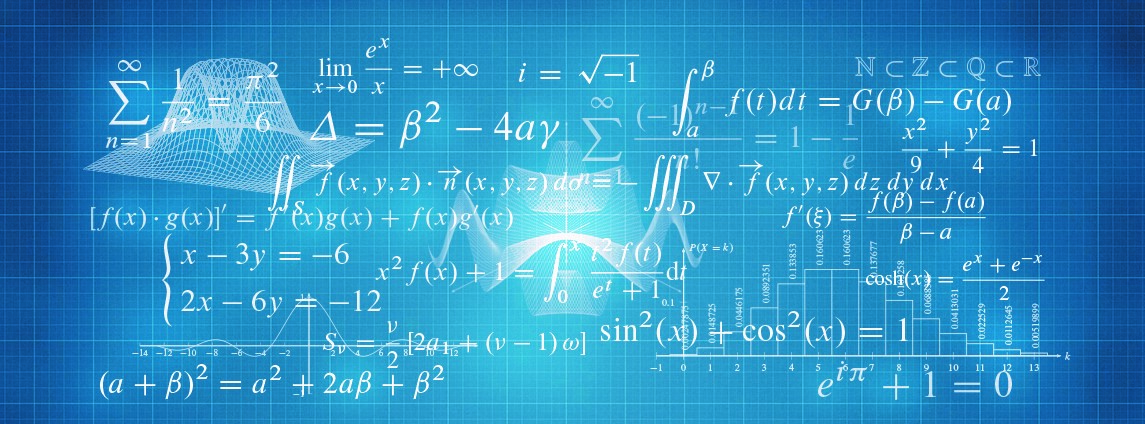
\includegraphics[width=17cm]{Kefalaio}};
\node[anchor=west,xshift=.1\paperwidth,yshift=.14\paperheight,rectangle]
{{\color{white}\fontsize{30}{20}\textbf{\textcolor{black}{\contour{white}{ΚΕΦΑΛΑΙΟ}}}}};
\node[anchor=west,xshift=.09\paperwidth,yshift=.08\paperheight,rectangle] {\fontsize{24}{20} {\color{black}{{\textcolor{black}{\contour{white}{\sc##1}}}}}};
%\fill[fill=black] (12.2,2) rectangle (14.8,4.7);
\node[anchor=west,xshift=.74\paperwidth,yshift=.11\paperheight,rectangle]
{{\color{white}\fontsize{80}{20}\textbf{\textit{\textcolor{white}{\contour{black}{\thechapter}}}}}};
\end{tikzpicture}
};
\end{tikzpicture}
}
\titlespacing*{\chapter}{0pt}{20pt}{30pt}
}
%------------------------------------------------


\usepackage[outline]{contour}
\newcommand{\regularchapter}{%
\titleformat{\chapter}[display]
{\normalfont\huge\bfseries}{\chaptertitlename\ \thechapter}{20pt}{\Huge##1}
\titlespacing*{\chapter}
{0pt}{-20pt}{40pt}
}

\apptocmd{\mainmatter}{\fancychapter}{}{}
\apptocmd{\backmatter}{\regularchapter}{}{}
\apptocmd{\frontmatter}{\regularchapter}{}{}

\titlespacing*{\section}
{0pt}{30pt}{0pt}
\usepackage{booktabs}
\usepackage{hhline}
\DeclareRobustCommand{\perthousand}{%
\ifmmode
\text{\textperthousand}%
\else
\textperthousand
\fi}


\contentsmargin{0cm}
\titlecontents{part}[-1pc]
{\addvspace{10pt}%
\bf\Large ΜΕΡΟΣ\quad }%
{}
{}
{\;\dotfill}%
%------------------------------------------
\titlecontents{chapter}[0pc]
{\addvspace{30pt}%
\begin{tikzpicture}[remember picture, overlay]%
\draw[fill=black,draw=black] (-.3,.5) rectangle (3.7,1.1); %
\pgftext[left,x=0cm,y=0.75cm]{\color{white}\sc\Large\bfseries Κεφάλαιο\ \thecontentslabel};%
\end{tikzpicture}\large\sc}%
{}
{}
{\hspace*{-2.3em}\hfill\normalsize Σελίδα \thecontentspage}%
\titlecontents{section}[2.4pc]
{\addvspace{1pt}}
{\contentslabel[\thecontentslabel]{2pc}}
{}
{\;\dotfill\;\small \thecontentspage}
[]
\titlecontents*{subsection}[4pc]
{\addvspace{-1pt}\small}
{}
{}
{\ --- \small\thecontentspage}
[ \textbullet\ ][]

\makeatletter
\renewcommand{\tableofcontents}{%
\chapter*{%
\vspace*{-20\p@}%
\begin{tikzpicture}[remember picture, overlay]%
\pgftext[right,x=12cm,y=0.2cm]{\Huge\sc\bfseries \contentsname};%
\draw[fill=black,draw=black] (9.5,-.75) rectangle (12.5,1);%
\clip (9.5,-.75) rectangle (15,1);
\pgftext[right,x=12cm,y=0.2cm]{\color{white}\Huge\bfseries \contentsname};%
\end{tikzpicture}}%
\@starttoc{toc}}
\makeatother

\usepackage[contents={},scale=1,opacity=1,color=black,angle=0]{background}

\newcommand\blfootnote[1]{%
\begingroup
\renewcommand\thefootnote{}\footnote{#1}%
\addtocounter{footnote}{-1}%
\endgroup
}
\usepackage{epstopdf}
\epstopdfsetup{update}
\usepackage{textcomp}

\titleformat{\section}
{\normalfont\Large\bf}%
{}{0em}%
{{\color{black}\titlerule[0pt]}\vskip-.2\baselineskip{\parbox[t]{\dimexpr\textwidth-2\fboxsep\relax}{\raggedright\strut\itshape{\LARGE{\thesection~#1}}\strut}}}[\vskip 0\baselineskip{\color{black}\titlerule[1pt]}]
\titlespacing*{\section}{0pt}{0pt}{30pt}

\newcommand{\methodologia}{\begin{center}
{\large \textbf{ΜΕΘΟΔΟΛΟΓΙΑ}}\\\vspace{-2mm}
\begin{tikzpicture}
\shade[left color=white, right color=black,] (-3cm,0) rectangle (0,.2mm);
\shade[left color=black, right color=white,] (0,0) rectangle (3cm,.2mm);   
\end{tikzpicture}
\end{center}}

\newcommand{\orismoi}{\begin{center}
\vspace{-3mm}{\large \textbf{\textcolor{\xrwma}{ΟΡΙΣΜΟΙ}}}\\\vspace{-2mm}
\begin{tikzpicture}
\shade[left color=white, right color=cyan!80!black,] (-3cm,0) rectangle (0,.2mm);
\shade[left color=cyan!80!black, right color=white,] (0,0) rectangle (3cm,.2mm);   
\end{tikzpicture}
\end{center}}
\newcommand{\thewrhmata}{\begin{center}
{\large \textbf{\textcolor{\xrwmath}{ΘΕΩΡΗΜΑΤΑ - ΠΟΡΙΣΜΑΤΑ - ΠΡΟΤΑΣΕΙΣ\\ΚΡΙΤΗΡΙΑ - ΙΔΙΟΤΗΤΕΣ}}}\\\vspace{-2mm}
\begin{tikzpicture}
\shade[left color=white, right color=\xrwmath,] (-5cm,0) rectangle (0,.2mm);
\shade[left color=\xrwmath, right color=white,] (0,0) rectangle (5cm,.2mm);   
\end{tikzpicture}
\end{center}}
\usepackage[labelfont={footnotesize,it,bf},font={footnotesize}]{caption}

%-------- ΠΙΝΑΚΕΣ ---------
\usepackage{booktabs}
%----------------------
%----- ΥΠΟΛΟΓΙΣΤΗΣ ----------
%\usepackage{calculator}
%----------------------------

%----- ΟΡΙΖΟΝΤΙΑ ΛΙΣΤΑ ------
\usepackage{xparse}
\newcounter{answers}
\renewcommand\theanswers{\arabic{answers}}
\ExplSyntaxOn
\NewDocumentCommand{\results}{m}
{
\seq_set_split:Nnn \l_results_a_seq {,}{#1}
\par\nobreak\noindent\setcounter{answers}{0}
\seq_map_inline:Nn \l_results_a_seq
{
\makebox[.18\linewidth][l]{\stepcounter{answers}\theanswers.~##1}\hfill
}
\par
}
\seq_new:N \l_results_a_seq
\ExplSyntaxOff
%----------------------------
%------ ΜΗΚΟΣ ΓΡΑΜΜΗΣ ΚΛΑΣΜΑΤΟΣ ---------
\DeclareRobustCommand{\frac}[3][0pt]{%
{\begingroup\hspace{#1}#2\hspace{#1}\endgroup\over\hspace{#1}#3\hspace{#1}}}
%----------------------------------------
\usepackage{microtype}
\usepackage{float}

\usepackage{caption}

%---- ΟΡΙΖΟΝΤΙΟ - ΚΑΤΑΚΟΡΥΦΟ - ΠΛΑΓΙΟ ΑΓΚΙΣΤΡΟ ------
\newcommand{\orag}[3]{\node at (#1)
{$ \overcbrace{\rule{#2mm}{0mm}}^{{\scriptsize #3}} $};}

\newcommand{\kag}[3]{\node at (#1)
{$ \undercbrace{\rule{#2mm}{0mm}}_{{\scriptsize #3}} $};}

\newcommand{\Pag}[4]{\node[rotate=#1] at (#2)
{$ \overcbrace{\rule{#3mm}{0mm}}^{{\rotatebox{-#1}{\scriptsize$#4$}}}$};}
%-----------------------------------------
\tikzstyle{pl}=[line width=0.3mm]
\tikzstyle{plm}=[line width=0.4mm]
%------- ΣΤΥΛ ΠΑΡΑΔΕΙΓΜΑΤΟΣ -------
\newcounter{paradeigma}[section]
\renewcommand{\theparadeigma}{\bf\arabic{paradeigma}\;:\;}   
\newcommand{\Paradeigma}[1]{\refstepcounter{paradeigma}\textcolor{black}{\textbf{ΠΑΡΑΔΕΙΓΜΑ\hspace{2mm}\theparadeigma\hspace{1mm}}} \MakeUppercase{\textbf{#1}}\\}{}
%-----------------------------------

%------- ΣΤΥΛ ΛΥΣΗΣ ------------------
\newcommand{\lysh}{{\textbf{ΛΥΣΗ}}}
%------------------------------------

%------ ΛΥΜΕΝΑ ΠΑΡΑΔΕΙΓΜΑΤΑ ΤΙΤΛΟΣ ---------
\newcommand{\Lymena}{\begin{center}
\begin{tikzpicture}
\path[left color=cyan!70!black,right color=cyan!80!black,middle color=cyan!80!white] (-7cm,-.6cm) rectangle (6.5cm,.6cm);
\node at (-.25cm,0) {\Large \textcolor{white}{\textbf{ΛΥΜΕΝΑ ΠΑΡΑΔΕΙΓΜΑΤΑ}}};  
\end{tikzpicture}
\end{center}}
%--------------------------------------

%--------- ΑΛΥΤΕΣ ΑΣΚΗΣΕΙΣ ΤΙΤΛΟΣ ----------
\newcommand{\Alyta}{\begin{center}
\begin{tikzpicture}
\path[left color=cyan!70!black,right color=cyan!80!black,middle color=cyan!80!white] (-7cm,-.6cm) rectangle (6.5cm,.6cm);
\node at (-.25cm,0) {\Large \textcolor{white}{\textbf{ΑΣΚΗΣΕΙΣ - ΠΡΟΒΛΗΜΑΤΑ}}};  
\end{tikzpicture}
\end{center}}
%--------------------------------------------
\usetikzlibrary{shadows,calc}
\usepackage{tcolorbox}
\tcbuselibrary{skins,theorems,breakable}
%---------- ΜΕΘΟΔΟΣ --------------
\newcounter{Methodos}[chapter]
\renewcommand{\theMethodos}{\thechapter.\arabic{Methodos}}
\newenvironment{Methodos}[2][\linewidth]
{\refstepcounter{Methodos}
\begin{tcolorbox}[breakable,
enhanced standard,
boxrule=0.7pt,titlerule=-.2pt,drop fuzzy shadow southeast=black!50,
width=\linewidth,
title style={color=white},
overlay unbroken and first={
\path[left color=cyan!70!black,right color=cyan,draw=black]
([yshift=-\pgflinewidth]frame.north west) to ([yshift=-5pt]title.south west)[rounded corners=2pt] -- ([xshift=-#2-15pt,yshift=-5pt]title.south east) to[rounded corners=2pt] ([xshift=-#2,yshift=-\pgflinewidth]frame.north east) -- cycle;
},
fonttitle=\bfseries,
before=\par\medskip\noindent,
after=\par\medskip,
toptitle=3pt,
top=11pt,topsep at break=-5pt,
colback=white,title={\large Μέθοδος \theMethodos} : {\textcolor{black}{\MakeUppercase{#1}}}]}
{\end{tcolorbox}}
%------------------------------------------
%---------- ΛΙΣΤΕΣ ----------------------
\newlist{bhma}{enumerate}{3}
\setlist[bhma]{label=\bf\textit{\arabic*\textsuperscript{o}\;Βήμα :},leftmargin=0cm,itemindent=1.5cm,ref=\bf{\arabic*\textsuperscript{o}\;Βήμα}}
\newlist{rlist}{enumerate}{3}
\setlist[rlist]{itemsep=0mm,label=\roman*.}


%----ΣΤΥΛ ΑΣΚΗΣΗΣ ----------
\newcounter{askhsh}[chapter]
\renewcommand{\theaskhsh}{\bf{{\large{\thechapter}}.\arabic{askhsh}}}   
\newcommand{\Askhsh}{\refstepcounter{askhsh}\textcolor{\xrwma}{{\theaskhsh}\hspace{1mm}}}{}
%---------------------------

\newlist{brlist}{enumerate}{3}
\setlist[brlist]{itemsep=0mm,label=\bf\roman*.}
\newlist{tropos}{enumerate}{3}
\setlist[tropos]{label=\bf\textit{\arabic*\textsuperscript{oς}\;Τρόπος :},leftmargin=0cm,itemindent=2.3cm,ref=\bf{\arabic*\textsuperscript{oς}\;Τρόπος}}
% Αν μπει το bhma μεσα σε tropo τότε
%\begin{bhma}[leftmargin=.7cm]
\newcommand{\tss}[1]{\textsuperscript{#1}}
\newcommand{\tssL}[1]{\MakeLowercase{\textsuperscript{#1}}}
%------------------------------------------
\setlength{\parindent}{0pt}
\setlist[itemize]{itemsep=0mm}
\tkzSetUpPoint[size=7,fill=white]
\newcommand{\twocolkentro}[1]{
\twocolumn[
\begin{@twocolumnfalse}
#1
\end{@twocolumnfalse}]}




\begin{document}
\title{\MakeUppercase{Άλγεβρα Α' Λυκείου}}
\pagestyle{empty}
\frontmatter
\begin{titlepage}
\newgeometry{left=2.5cm,top=2.5cm} %defines the geometry for the titlepage
\pagecolor{white}
\begin{center}
{\large Σπύρος Φρόνιμος\\Μαθηματικός}
\end{center}
\noindent
\par
\noindent
\mbox{}\\\\
\begin{center}
\textbf{\fontsize{20}{40}\selectfont{Άλγεβρα}}\par\mbox{}\\\vspace{-3mm}
\textbf{\fontsize{20}{40}\selectfont{Α' ΛΥΚΕΙΟΥ}}\par\mbox{}\\
\vspace{-4mm}
\rule{12cm}{0.1mm}\\
\vspace{3mm}
{\fontsize{15}{15}\MakeUppercase{τύποι ορισμοί θεωρήματα και}}\\
\vspace{.7mm}
{\fontsize{15}{15}\MakeUppercase{βασική μεθοδολογία της}}\\
\vspace{.7mm}
{\fontsize{15}{15}\MakeUppercase{Άλγεβρας της Α' ΛΥΚΕΙΟΥ}}\\
\rule{12cm}{0.1mm}\\
\end{center}
\vspace{3cm}
\begin{flushright}
\begin{itemize}
\item 100 Ορισμοί
\item 250 Θεωρήματα
\item 400 Μέθοδοι για λύση ασκήσεων
\item 200 Λυμένα παραδείγματα
\item 500 Άλυτες ασκήσεις και προβλήματα
\item 200 Επαναληπτικά θέματα
\item Απαντήσεις ασκήσεων
\end{itemize}
\end{flushright}

\vfill
\noindent
\color{black}
\begin{center}
{\large{ΕΚΔΟΣΕΙΣ \_\_\_\_\_}\\
\large{ΚΕΡΚΥΡΑ 2015}}
\vskip\baselineskip
\end{center}
\hbox{ % Horizontal box
\hspace*{0.2\textwidth} % Whitespace to the left of the title page
\rule{1pt}{\textheight} % Vertical line
\hspace*{0.05\textwidth} % Whitespace between the vertical line and title page text
\parbox[b]{0.75\textwidth}{ % Paragraph box which restricts text to less than the width of the page

{\textbf{ΜΑΘΗΜΑΤΙΚΑ}\\\textbf{Β΄ Λύκείου}\\\\\noindent \textbf{Σπύρος Φρόνιμος - Μαθηματικός}\\e-mail : spyrosfronimos@gmail.com\\[0.5\baselineskip]
Σελίδες : ...\\
ΙΣΒΝ : ...\\
Εκδόσεις : ...\\
\textcopyright Copyright 2015}\\[2\baselineskip] % Title
{Φιλολογική Επιμέλεια :\\\textbf{Μαρία Πρεντουλή}}
{- e-mail : predouli@yahoo.com}\\[0.5\baselineskip]
{Επιστημονική Επιμέλεια :}{\textbf{Σπύρος Φρόνιμος}}\\[0.5\baselineskip]
{Εξώφυλλο : \\\textbf{Δημήτρης Πρεντουλής}}\\[1\baselineskip] % Tagline or further description
% Author name

\vspace{.4\textheight} % Whitespace between the title block and the publisher
{Πνευματικά Δικαιώματα : ...}\\[\baselineskip]}}
\vspace*{2\baselineskip}
\newpage
\mbox{}\\\\\\\\\\\\
\hspace*{0.75\textwidth}
\textit{{\large Στη γυναίκα μου.}}
\newpage
\mbox{}
\newpage
\mbox{}
{\LARGE \textbf{Πρόλογος}}\\\\\\\\

Το βιβλίο περιέχει συγκεντρωμένη όλη τη θεωρία των μαθηματικών όλων των τάξεων του γυμνασίου και του λυκείου γραμμένη αναλυτικά και κατανοητά.\\\\
Ειδικότερα ο αναγνώστης θα βρει\\
\vspace{-.4cm}
\begin{itemize}
\item Ορισμούς
\item Θεωρήματα
\item Τυπολόγιο
\item Μεθοδολογία
\end{itemize}
Σκοπό έχει να αποτελέσει ένα χρήσιμο βοήθημα για μικρούς ή μεγάλους μαθητές όπου μπορούν να έχουν όλη τη θεωρία της χρονιάς τους συγκεντρωμένη, χρήσιμη για επανάληψη και διαγωνίσματα, αλλά και να μπορούν εύκολα να καλύψουν τυχόν κενά από προηγούμενες τάξεις.\\\\\\
Θέλω να ευχαριστήσω όλους όσους βοήθησαν.
\newpage
\end{titlepage}
\restoregeometry % restores the geometry
\tableofcontents
\mainmatter
\pagestyle{fancy}
\chapter{Σύνολα - Πιθανότητες} 
\section{Σύνολα}
\orismoi
\Orismos{Σύνολο} Σύνολο ονομάζεται μια συλλογή όμοιων αντικειμένων, τα οποία είναι καλά ορισμένα και διακριτά μεταξύ τους.
\begin{itemize}[itemsep=0mm]
\item Τα αντικείμενα ενός συνόλου ονομάζονται \textbf{στοιχεία}.
\item Τα σύνολα τα συμβολίζουμε με ένα κεφαλαίο γράμμα.
\end{itemize}
\textbf{ΒΑΣΙΚΑ ΣΥΝΟΛΑ ΑΡΙΘΜΩΝ}
\begin{enumerate}[itemsep=0mm,label=\bf\arabic*.]
\item \textbf{Φυσικοί Αριθμοί} : Το σύνολο των αριθμών από το 0 εως το άπειρο όπου κάθε αριθμός έχει διαφορά μιας μονάδας από τον προηγούμενο. Συμβολίζεται με $ \mathbb{N} $ και είναι : $ \mathbb{N}=\{0,1,2,\ldots\} $.
\item \textbf{Ακέραιοι Αριθμοί} : Το σύνολο των φυσικών αριθμών μαζί με τους αντίθετους τους. Συμβολίζεται με $ \mathbb{Z} $ και είναι : $ \mathbb{Z}=\{\ldots,-2,-1,0,1,2,\ldots\} $.
\item \textbf{Ρητοί Αριθμοί} : Όλοι οι αριθμοί που μπορούν να γραφτούν με τη μορφή κλάσματος με ακέραιους όρους. Συμβολίζεται με $ \mathbb{Q} $ και είναι : $ \mathbb{Q}=\LEFTRIGHT\{\}{\left. \frac{a}{\beta}\right|a,\beta\in\mathbb{Z},\beta\neq0\;} $.
\item \textbf{Άρρητοι Αριθμοί} : Κάθε αριθμός ο οποίος δεν είναι ρητός. Κατά κύριο λόγο, άρρητοι αριθμοί είναι οι ρίζες που δεν έχουν ρητό αποτέλεσμα, ο αριθμός $ \pi $ κ.τ.λ.
\item \textbf{Πραγματικοί Αριθμοί} : Οι ρητοί μαζί με το σύνολο των άρρητων μας δίνουν τους πραγματικούς αριθμούς, όλους τους αριθμούς που γνωρίζουμε. Συμβολίζεται με $ \mathbb{R} $ και είναι : $ \mathbb{R}= $ $ \{ $όλοι οι αριθμοί$ \} $.
\end{enumerate}
Τα παραπάνω σύνολα χωρίς το μηδενικό τους στοιχείο συμβολίζονται αντίστοιχα με $ \mathbb{N}^*,\mathbb{Z}^*,\mathbb{Q}^*,\mathbb{R}^*$.\\\\
\Orismos{Ίσα σύνολα} Ίσα ονομάζονται δύο σύνολα $ A,B $ τα οποία έχουν ακριβώς τα ίδια στοιχεία. Ισοδύναμα, τα σύνολα $ Α,Β $ λέγονται ίσα εαν ισχύουν οι σχέσεις :
\begin{enumerate}[itemsep=0mm]
\item Κάθε στοιχείο του $ A $ είναι και στοιχείο του $ B $
\item Κάθε στοιχείο του $ B $ είναι και στοιχείο του $ A $.
\end{enumerate}
\Orismos{Υποσύνολο} Ένα σύνολο $ A $ λέγεται υποσύνολο ενός συνόλου $ B $ όταν κάθε στοιχείο του $ A $ είναι και στοιχείο του $ B $. Συμβολίζεται με τη χρήση του συμβόλου $ \subseteq $ ως εξής :
\[ A\subseteq B \]
\Orismos{Κενό σύνολο} Κενό ονομάζεται το σύνολο που δεν έχει κανένα στοιχείο. Συμβολίζεται με $ \varnothing $ ή $ \left\lbrace \right\rbrace  $.\\\\
\Orismos{Βασικό σύνολο} Βασικό ονομάζεται το σύνολο το οποίο περιέχει όλα τα στοιχεία που μπορούμε να επιλέξουμε, από τα οποία φτιάχνουμε άλλα σύνολα. Συμβολίζεται με $ \varOmega $.\\\\
\Orismos{Πράξεισ μεταξύ συνόλων}
\vspace{-4mm}
\begin{enumerate}[label=\bf\arabic*.,itemsep=0mm]
\item \textbf{Ένωση}\\
\begin{minipage}{\linewidth}
\begin{WrapText1}{8}{3.5cm}
\vspace{-5mm}
\begin{venndiagram2sets}[tikzoptions={scale=.7,samples=100},shade=\xrwma!50,labelNotAB={$ \varOmega $}]
\fillA \fillB
\end{venndiagram2sets}
\end{WrapText1}
Ένωση δύο υποσυνόλων $ A,B $ ενός βασικού συνόλου $ \varOmega $ ονομάζεται το σύνολο των στοιχείων του $ \varOmega $ τα οποία ανήκουν σε τουλάχιστον ένα από τα σύνολα $ A $ και $ B $. Συμβολίζεται με $ A\cup B $.  \[ A\cup B=\left\lbrace x\in\varOmega\left| x\in A \textrm{ ή } x\in B\right.\right\rbrace \]
Η ένωση των συνόλων $ A $ και $ B $ περιέχει τα κοινά και μή κοινά στοιχεία των δύο συνόλων. Τα κοινά στοιχεία αναγράφονται μια φορά.\end{minipage}
\item \textbf{Τομή}\\
\begin{minipage}{\linewidth}
\begin{WrapText1}{7}{3.5cm}
\vspace{-5mm}
\begin{venndiagram2sets}[tikzoptions={scale=.7},shade=\xrwma!50,labelNotAB={$ \varOmega $}]
\fillACapB
\end{venndiagram2sets}
\end{WrapText1}
Τομή δύο υποσυνόλων $ A,B $ ενός βασικού συνόλου $ \varOmega $ ονομάζεται το σύνολο των στοιχείων του $ \varOmega $ τα οποία ανήκουν και στα δύο σύνολα $ A $ και $ B $. Συμβολίζεται με $ A\cap B $. \[ A\cap B=\left\lbrace x\in\varOmega\left| x\in A \textrm{ και } x\in B\right.\right\rbrace \]
Η τομή των συνόλων $ A $ και $ B $ περιέχει μόνο τα κοινά στοιχεία των δύο συνόλων.\end{minipage}
\item \textbf{Συμπλήρωμα}\\
\begin{minipage}{\linewidth}
\begin{WrapText1}{8}{3.5cm}
\vspace{-5mm}
\begin{tikzpicture}[scale=.77]
\filldraw[fill=\xrwma!50] (-2,-2) rectangle (2.6,1);
\scope % A \cap B
\fill[white] (-.45,-.5) circle (1.1);
\draw[black] (-.45,-.5) circle (1.1);
\endscope
\tkzText(-1.6,-1.6){$ \varOmega $}
\tkzText(-.45,.3){$ A $}
\end{tikzpicture}
\end{WrapText1}
Συμπλήρωμα ενός συνόλου $ A $ ονομάζεται το σύνολο των στοιχείων του βασικού συνόλου $ \varOmega $ τα οποία \textbf{δεν} ανήκουν στο σύνολο $ A $. Συμβολίζεται με $ A' $. \[ A'=\left\lbrace x\in\varOmega\left| x\notin A\right.\right\rbrace \] Ονομάζεται συμπλήρωμα του $ Α $ γιατί η ένωσή του με το σύνολο αυτό μας δίνει το βασικό σύνολο $ \varOmega $.\end{minipage}
\item \textbf{Διαφορά}\\
\begin{minipage}{\linewidth}
\begin{WrapText1}{8}{3.5cm}
\vspace{-5mm}
\begin{venndiagram2sets}[tikzoptions={scale=.7},shade=\xrwma!50,labelNotAB={$ \varOmega $}]
\fillANotB
\end{venndiagram2sets}
\end{WrapText1}
Διαφορά ενός συνόλου $ B $ από ένα σύνολο $ A $ ονομάζεται το σύνολο των στοιχείων του βασικού συνόλου $ \varOmega $ τα οποία ανήκουν μόνο στο σύνολο $ A $, το πρώτο σύνολο της διαφοράς. Συμβολίζεται με $ A-B $. \[ A-B=\left\lbrace x\in\varOmega\left| x\in A\textrm{ και }x\notin B\right. \right\rbrace  \]
\end{minipage}
\end{enumerate}\mbox{}\\\\
\thewrhmata
\Thewrhma{Ιδιότητεσ Υποσυνολου}
Για οποιαδήποτε σύνολα $ A,B,\varGamma $ ισχύουν οι ακόλουθες ιδιότητες που αφορούν τη σχέση του υποσυνόλου :
\begin{rlist}
\item Για κάθε σύνολο $ A $ ισχύει : $ A\subseteq A $.
\item Αν $ A\subseteq B $ και $ B\subseteq \varGamma $ τότε $ A\subseteq \varGamma $.
\item Αν $ A\subseteq B $ και $ B\subseteq A $ τότε $ A=B $.
\end{rlist}
\section{Δειγματικός χώρος - Ενδεχόμενα}
\orismoi
\Orismos{Πείραμα τύχησ} Πείραμα τύχης ονομάζεται κάθε πείραμα του οποίου το αποτέλεσμα δεν μπορεί να προβλευθεί με απόλυτη βεβαιότητα όσες φορές κι αν αυτό επαναληφθεί, κάτω από τις ίδιες συνθήκες.\\\\
\Orismos{Δειγματικόσ Χώροσ} Δειγματικός χώρος ονομάζεται το σύνολο το οποίο περιέχει όλα τα πιθανά αποτελέσματα ενός πειράματος τύχης. Ο δειγματικός αποτελέι βασικό σύνολο. \[ \varOmega=\left\lbrace \omega_1,\omega_2,\ldots,\omega_\nu \right\rbrace \]
\Orismos{Ενδεχόμενο} Ενδεχόμενο ονομάζεται το σύνολο το οποίο περιέχει ένα ή περισσότερα στοιχεία του δειγματικού χώρου ενός πειράματος.
\begin{itemize}[itemsep=0mm]
\item Κάθε ενδεχόμενο είναι υποσύνολο του δειγματικού του χώρου.
\item Συμβολίζεται με κεφαλαίο γράμμα π.χ. : $ A,B,\ldots $
\item Τα ενδεχόμενα που έχουν ένα στοιχείο ονομάζονται \textbf{απλά} ενδεχόμενα, ενώ αν περιέχουν περισσότερα στοιχεία ονομάζονται \textbf{σύνθετα}.
\item Εαν το αποτέλεσμα ενός πειράματος είναι στοιχείο ενός ενδεχομένου τότε το ενδεχόμενο \textbf{πραγματοποιείται}.
\item Τα στοιχεία ενός ενδεχομένου ονομάζονται ευνοϊκές περιπτώσεις.
\item Ο δειγματικός χώρος $ \varOmega $ ονομάζεται \textbf{βέβαιο} ενδεχόμενο, ενώ το κενό σύνολο ονομάζεται \textbf{αδύνατο} ενδεχόμενο.
\item Εαν δύο ενδεχόμενα $ A,B $ δεν έχουν κοινά στοιχεία τότε ονομάζονται \textbf{ασυμβίβαστα} ή ξένα μεταξύ τους δηλαδή : \[ A,B \textrm{ ασυμβίβαστα }\Leftrightarrow A\cap B=\varnothing \]
\end{itemize}\mbox{}\\
\Orismos{πράξεισ με ενδεχόμενα}
Οι πράξεις μεταξύ ενδεχομένων ορίζονται ακριβώς όπως και οι πράξεις μεταξύ συνόλων. Κάθε ορισμός προσαρμόζεται ώστε να περιγράψει την ισχύ του ενδεχομένου σε κάθε περίπτωση.
\begin{enumerate}[label=\bf\arabic*.,itemsep=0mm]
\item \textbf{Ένωση}\\
Ένωση δύο ενδεχομένων $ A,B $ ονομάζεται το ενδεχόμενο το οποίο περιέχει τα κοινά και μη κοινά στοιχεία των δύο ενδεχομένων. Η ένωση πραγματοποιείται όταν πραγματοποιείται τουλάχιστον ένα από τα ενδεχόμενα $ A $ ή $ B $. \[ x\in A\cup B\Leftrightarrow x\in A \textrm{ ή }x\in B \]
\item \textbf{Τομή}\\
Τομή δύο ενδεχομένων $ A,B $ ονομάζεται το ενδεχόμενο το οποίο περιέχει τα κοινά στοιχεία των δύο ενδεχομένων. Η τομή πραγματοποιείται όταν πραγματοποιούνται συγχρόνως και τα δύο ενδεχόμενα $ A $ και $ B $. \[ x\in A\cap B\Leftrightarrow x\in A \textrm{ και }x\in B \]
\item \textbf{Συμπλήρωμα}\\Συμπλήρωμα ενός ενδεχομένου $ A $ ονομάζεται το ενδεχόμενο το οποίο περιέχει τα στοιχεία εκείνα τα οποία \textbf{δεν} ανήκουν στο σύνολο $ A $. Το συμπλήρωμα πραγματοποιείται όταν δεν πραγματοποιείται το $ A $. \[ x\in A'\Leftrightarrow x\notin A\]
\item \textbf{Διαφορά}\\
Διαφορά ενός ενδεχομένου $ A $ από ένα ενδεχόμενο $ B $ ονομάζεται το ενδεχόμενο που περιέχει τα στοιχεία που ανήκουν μόνο στο ενδεχόμενο $ A $. Η διαφορά πραγματοποιείται όταν πραγματοποιείται μόνο το ενδεχόμενο $ A $. \[ x\in A-B\Leftrightarrow x\in A \textrm{ και }x\notin B \]
\end{enumerate}
Στον παρακάτω πίνακα φαίνονται τα ενδεχόμενα, οι πράξεις μεταξύ δύο ενδεχομένων $ A,B $, οι συμβολισμοί τους, λεκτική περιγραφή καθώς και διάγραμμα για κάθε περίπτωση.
\begin{center}
\begin{longtable}{c>{\centering}m{2cm}>{\centering}m{3.5cm} c}
\hline \rule[-2ex]{0pt}{5.5ex} \textbf{Συμβολισμός} & \textbf{Ενδεχόμενο} & \textbf{Περιγραφή} & \textbf{Διάγραμμα} \\ 
\hhline{====} \rule[-2ex]{0pt}{8.5ex} $ x\in A $ & Ενδεχόμενο Α & Το ενδεχόμενο $ A $ πραγματοποιείται. & \parbox[c]{22mm}{\mbox{}\\\begin{tikzpicture}[scale=.438]
\draw (-2,-2) rectangle (2.6,1);
\scope % A \cap B
\fill[\xrwma!50] (-.45,-.5) circle (1.1);
\draw[black] (-.45,-.5) circle (1.1);
\endscope
\tkzText(-1.6,-1.6){{\scriptsize $ \varOmega $}}
\tkzText(-.45,.1){{\scriptsize $ A $}}
\end{tikzpicture}} \\ 
\rule[-2ex]{0pt}{8.5ex} $ x\in A' $ & Συμπλήρωμα του $ A $ & Το ενδεχόμενο $ A $ \textbf{δεν} πραγματοποιείται. & \parbox[c]{22mm}{\mbox{}\\\begin{tikzpicture}[scale=.438]
\filldraw[fill=\xrwma!50] (-2,-2) rectangle (2.6,1);
\scope % A \cap B
\fill[white] (-.45,-.5) circle (1.1);
\draw[black] (-.45,-.5) circle (1.1);
\endscope
\tkzText(-1.6,-1.6){{\scriptsize $ \varOmega $}}
\tkzText(-.45,.1){{\scriptsize $ A $}}
\end{tikzpicture}} \\ 
\rule[-2ex]{0pt}{8.5ex} $ x\in A\cup B $ & Ένωση του $ A $ με το $ B $ & Πραγματοποιείται ένα \textbf{τουλάχιστον} από τα ενδεχόμενα $ A $ και $ B $. & \parbox[c]{22mm}{\mbox{}\\\begin{venndiagram2sets}[tikzoptions={scale=.4},shade=\xrwma!50,labelA={{\scriptsize $ A $}},labelB={{\scriptsize $ B $}},labelNotAB={{\scriptsize $ \varOmega $}}]
\fillA \fillB
\end{venndiagram2sets}} \\ 
\rule[-2ex]{0pt}{8.5ex} $ x\in A\cap B $ & Τομή του $ A $ με το $ B $ & Πραγματοποιούνται \textbf{συγχρόνως} τα ενδ. $ A $ και $ B $. & \parbox[c]{22mm}{\mbox{}\\\begin{venndiagram2sets}[tikzoptions={scale=.4},shade=\xrwma!50,labelA={{\scriptsize $ A $}},labelB={{\scriptsize $ B $}},labelNotAB={{\scriptsize $ \varOmega $}}]
\fillACapB
\end{venndiagram2sets}} \\ 
\rule[-2ex]{0pt}{8.5ex} $ x\in A-B $ & Διαφορά του $ B $ απ' το $ A $ & Πραγματοποιείται \textbf{μόνο} το ενδεχόμενο $ A $. & \parbox[c]{22mm}{\mbox{}\\\begin{venndiagram2sets}[tikzoptions={scale=.4},shade=\xrwma!50,labelA={{\scriptsize $ A $}},labelB={{\scriptsize $ B $}},labelNotAB={{\scriptsize $ \varOmega $}}]
\fillANotB
\end{venndiagram2sets}} \\ 
\rule[-2ex]{0pt}{8.5ex} $ x\in B-A $ & Διαφορά του $ A $ απ' το $ B $ & Πραγματοποιείται \textbf{μόνο} το ενδεχόμενο $ B $. & \parbox[c]{22mm}{\mbox{}\\\begin{venndiagram2sets}[tikzoptions={scale=.4},shade=\xrwma!50,labelA={{\scriptsize $ A $}},labelB={{\scriptsize $ B $}},labelNotAB={{\scriptsize $ \varOmega $}}]
\fillBNotA
\end{venndiagram2sets}} \\ 
\rule[-2ex]{0pt}{8.5ex} $ x\in\left(A-B\right)\cup\left(B-A\right) $ & Ένωση διαφορών & Πραγματοποιείται \textbf{μόνο} ένα από τα δύο ενδ. (ή μόνο το $ A $ ή μόνο το $ B $). & \parbox[c]{22mm}{\mbox{}\\\begin{venndiagram2sets}[tikzoptions={scale=.4},shade=\xrwma!50,labelA={{\scriptsize $ A $}},labelB={{\scriptsize $ B $}},labelNotAB={{\scriptsize $ \varOmega $}}]
\fillANotB \fillBNotA
\end{venndiagram2sets}} \\ 
\rule[-2ex]{0pt}{8.5ex} \begin{minipage}{2.8cm}
\begin{center}
$ A\subseteq B $\\
$ x\in A\Rightarrow x\in B $
\end{center}
\end{minipage} & $ A $ υποσύνολο του $ B $ & Η πραγματοποίηση του $ A $ συνεπάγεται πραγμ/ση του $ B $. & \parbox[c]{22mm}{\mbox{}\\\begin{tikzpicture}[scale=.438]
\draw (-2,-2) rectangle (2.6,1);
\scope % A \cap B
\filldraw[fill=\xrwma!50] (-.45,-.5) circle (1.1);
\draw[fill=\xrwma!50] (-.5,-.5) circle (.7);
\endscope
\tkzText(-1.6,-1.6){{\scriptsize $ \varOmega $}}
\tkzText(.9,.1){{\scriptsize $ B $}}
\tkzText(-.45,-.2){{\scriptsize $ A $}}
\end{tikzpicture}} \\ 
\rule[-2ex]{0pt}{8.5ex} $ x\in\left(A\cap B\right)' $ & Συμπλήρωμα τομής & \textbf{Δεν} πραγματοποιούνται \textbf{συγχρονως} τα ενδ. $ A $ και $ B $. & \parbox[c]{22mm}{\mbox{}\\\begin{venndiagram2sets}[tikzoptions={scale=.4},shade=\xrwma!50,labelA={{\scriptsize $ A $}},labelB={{\scriptsize $ B $}},labelNotAB={{\scriptsize $ \varOmega $}}]
\fillNotAorNotB
\end{venndiagram2sets}}\\
\rule[-2ex]{0pt}{8.5ex} $ x\in\left(A\cup B\right)' $ & Συμπλήρωμα ένωσης & Δεν πραγματοποιείται \textbf{κανένα} από τα ενδ. $ A $ και $ B $. & \parbox[c]{22mm}{\mbox{}\\\begin{venndiagram2sets}[tikzoptions={scale=.4},shade=\xrwma!50,labelA={{\scriptsize $ A $}},labelB={{\scriptsize $ B $}},labelNotAB={{\scriptsize $ \varOmega $}}]
\fillNotAorB
\end{venndiagram2sets}}\\
\rule[-2ex]{0pt}{8.5ex} $ x\in\left( A-B\right)'  $ & Συμπλήρωμα διαφοράς & \textbf{Δεν} πραγματοποιείται αποκλειστικά το ενδεχόμενο $ A $. & \parbox[c]{22mm}{\mbox{}\\\begin{venndiagram2sets}[tikzoptions={scale=.4},shade=\xrwma!50,labelA={{\scriptsize $ A $}},labelB={{\scriptsize $ B $}},labelNotAB={{\scriptsize $ \varOmega $}}]
\fillNotAorB \fillB
\end{venndiagram2sets}} \\
\rule[-2ex]{0pt}{8.5ex} $ x\in \left(B-A\right)'  $ & Συμπλήρωμα διαφοράς & \textbf{Δεν} πραγματοποιείται αποκλειστικά το ενδεχόμενο $ B $. & \parbox[c]{22mm}{\mbox{}\\\begin{venndiagram2sets}[tikzoptions={scale=.4},shade=\xrwma!50,labelA={{\scriptsize $ A $}},labelB={{\scriptsize $ B $}},labelNotAB={{\scriptsize $ \varOmega $}}]
\fillNotAorB \fillA
\end{venndiagram2sets}} \\
\rule[-2ex]{0pt}{8.5ex} $ x\in\left( \left(A-B\right)\cup\left(B-A\right)\right)'  $ & Συμπλήρωμα ένωσης διαφορών & \textbf{Δεν} πραγματοποιείται αποκλειστικά ένα από τα δύο ενδ. (ή κανένα ή και τα δύο). & \parbox[c]{22mm}{\mbox{}\\\begin{venndiagram2sets}[tikzoptions={scale=.4},shade=\xrwma!50,labelA={{\scriptsize $ A $}},labelB={{\scriptsize $ B $}},labelNotAB={{\scriptsize $ \varOmega $}}]
\fillNotAorB \fillACapB
\end{venndiagram2sets}} \\
\rule[-1ex]{0pt}{0ex} &&&\\
\hline
\end{longtable}
\end{center}
\section{Πιθανότητες}
\Orismos{Κλασικόσ Ορισμόσ Πιθανότητασ}
Πιθανότητα ενός ενδεχομένου $ A=\{a_1,a_2,\ldots,a_\kappa\} $ ενός δειγματικού χώρου $ \varOmega $ ονομάζεται ο λόγος του πλήθους των ευνοϊκών περιπτώσεων του $ A $ προς το πλήθος όλων των δυνατών περιπτώσεων.
\[ P(A)=\frac{N(A)}{N(\varOmega)} \]
\begin{itemize}[itemsep=0mm]
\item Ο παραπάνω ορισμός ονομάζεται \textbf{κλασικός ορισμός} της πιθανότητας και εφαρμόζεται όταν το ενδεχόμενο $ A $ αποτελείται από ισοπίθανα απλά ενδεχόμενα $ \{a_i\}\ ,\ i=1,2,\ldots,\kappa $.
\item Το πλήθος των στοιχείων ενός ενδεχομένου $ A $ συμβολίζεται με $ N(A) $.
\end{itemize}
\Orismos{Αξιωματικός Ορισμός Πιθανότητας}
Η πιθανότητα ενός ενδεχομένου $ A=\{a_1,a_2,\ldots,a_\kappa\} $ ενός δειγματικού χώρου $ \varOmega=\{\omega_1,\omega_2,\ldots,\omega_\nu\} $ ορίζεται ώς το άθροισμα των πιθανοτήτων $ P(a_i)\ ,\ i=1,2,\ldots,\nu $ των απλών ενδεχομένων του.
\[ P(A)=P(a_1)+P(a_2)+\ldots+P(a_\kappa) \]
\begin{itemize}[itemsep=0mm]
\item Για κάθε στοιχείο $ \omega_i\ ,\ i=1,2,\ldots,\nu $ του δειγματικού χώρου $ \varOmega $ ονομάζουμε τον αριθμό $ P(\omega_i) $ πιθανότητα του ενδεχομένου $ \{\omega_i\} $.
\item Ο παραπάνω ορισμός ονομάζεται \textbf{αξιοματικός ορισμός} της πιθανότητας και εφαρμόζεται όταν το ενδεχόμενο $ A $ δεν αποτελείται από ισοπίθανα απλά ενδεχόμενα $ \{a_i\}\ ,\ i=1,2,\ldots,\kappa $.
\end{itemize}
\thewrhmata
\Thewrhma{Ιδιότητες Πιθανοτήτων}
Από τον κλασικό ορισμό της πιθανότητας προκύπτουν οι παρακάτω ιδιότητες :
\begin{rlist}
\item Πιθανότητα κενού συνόλου : $ P(\varnothing)=0 $.
\item Πιθανότητα δειγματικού χώρου : $ P(\varOmega)=1 $.
\item Για κάθε ενδεχόμενο $ A $ ισχύει : $ 0\leq P(A)\leq1 $.
\end{rlist}
\Thewrhma{Κανόνες λογισμού πιθανοτήτων}
Οι παρακάτω ιδιότητες μας δείχνουν τις σχέσεις με τις οποίες συνδέονται οι πιθανότητες οποιονδήποτε ενδεχομένων $ A,B $ με τις πιθανότητες των ενδεχομένων των πράξεων που περιέχουν τα ενδεχόμενα αυτά.
\begin{center}
\begin{tabular}{cc}
\hline \rule[-2ex]{0pt}{5.5ex} \textbf{Ενδεχόμενο} & \textbf{Πιθανότητα} \\ 
\hhline{==} \rule[-2ex]{0pt}{7.5ex} Ένωση & $ P(a\cup B)=\ccases{P(A)+P(B)-P(A\cap B)\ \ ,\ \ \textrm{αν }A\cap B\neq\varnothing\\
P(A)+P(B)\ \ ,\ \ \textrm{αν }A\cap B=\varnothing} $ \\ 
 \rule[-2ex]{0pt}{5.5ex} Συμπλήρωμα & $ P(A')=1-P(A) $ \\ 
 \hhline{~-}\rule[-2ex]{0pt}{5.5ex} \multirow{3}{*}{Διαφορά} & $ P(A-B)=P(A)-P(A\cap B) $ \\ 
\rule[-2ex]{0pt}{5.5ex}  & $ P(B-A)=P(B)-P(A\cap B) $ \\ 
   \hhline{~-}\rule[-2ex]{0pt}{5.5ex} Υποσύνολο & $ A\subseteq B\Rightarrow P(A)\leq P(B) $ \\ 
\hline 
\end{tabular} 
\end{center}\mbox{}\\
\Thewrhma{Ανισότητες μεtαξύ πιθανοτήτων}
Μεταξύ των πιθανοτήτων δύο οποιονδήποτε ενδεχομένων $ A,B $ καθώς και των ενδεχομένων που προκύπτουν από πράξεις που τα περιέχουν, ισχύουν οι ακόλουθες ανισότητες.
\begin{multicols}{3}
\begin{rlist}
\item $ P(A)\leq P(A\cup B) $
\item $ P(B)\leq P(A\cup B) $
\item $ P(A\cap B)\leq P(A) $
\item $ P(A\cap B)\leq P(B) $
\item $ P(A\cap B)\leq P(A\cup B) $
\item $ P(A-B)\leq P(A) $
\item $ P(B-A)\leq P(B) $
\item $ P(A-B)\leq P(A\cup B) $
\item $ P(B-A)\leq P(A\cup B) $
\end{rlist}
\end{multicols}
\chapter{Πραγματικοί αριθμοί}
\section{Πράξεις πραγματικών αριθμών}
\orismoi
\Orismos{Άξονασ των πραγματικών αριθμών}
Ο άξονας των πραγματικών αριθμών είναι μια αριθμημένη ευθεία στην οποία μπορούν να τοποθετηθούν όλοι οι πραγματικοί αριθμοί σε αύξουσα σειρά από τα αριστερά προς τα δεξιά. \textbf{Αρχή} του άξονα είναι το σημείο $ O $ στο οποίο βρίσκεται ο αριθμός $ 0 $.
\begin{center}
\begin{tikzpicture}
\tkzInit[xmin=-4,xmax=4]
\draw[-latex] (-5,0) -- coordinate (x axis mid) (5.4,0) node[right,fill=white] {{\footnotesize $ x $}};
\foreach \x in {-5,-4,-3,...,5}
\draw (\x,.5mm) -- (\x,-.5mm) node[anchor=north,fill=white] {{\scriptsize \x}};
\draw[latex-|] (-5,0.7) --  (-0.02,0.7);
\draw[|-latex] (0.02,0.7) --  (5,0.7);
\tkzText(-2,0.85){Αρνητικοί Αριθμοί}
\tkzText(2,0.85){Θετικοί Αριθμοί}
\tkzDefPoint(3,0){A}
\tkzDefPoint(1.4142,0){B}
\tkzDefPoint(-1.5,0){C}
\tkzDefPoint(-2.7,0){D}
\tkzDrawPoints[size=7,fill=white](A,B,C,D)
\tkzLabelPoint[above](A){{\scriptsize $ A(3) $}}
\tkzLabelPoint[above](B){{\scriptsize $ B\left(\!\! \sqrt{2}\right)  $}}
\tkzLabelPoint[above](C){{\scriptsize $ \varGamma\left(-\frac{3}{2} \right)  $}}
\tkzLabelPoint[above](D){{\scriptsize $ \varDelta(-2{,}7) $}}
\end{tikzpicture}
\end{center}
\begin{itemize}[itemsep=0mm]
\item Η θέση ενός αριθμού πάνω στην ευθεία σχεδιάζεται με ένα σημείο.
\item Ο αριθμός που βρίσκεται στη θέση αυτή ονομάζεται \textbf{τετμημένη} του σημείου.
\end{itemize}
\Orismos{Δύναμη πραγματικου αριθμου}
Δύναμη ενός πραγματικού αριθμού $ a $ ονομάζεται το γινόμενο $ \nu $ ίσων παραγόντων του αριθμού αυτού. Συμβολίζεται με $ a^\nu $ όπου $ \nu\in\mathbb{N} $ είναι το πλήθος των ίσων παραγόντων. 
\[ \undercbrace{a\cdot a\cdot\ldots a}_{\nu\textrm{ παράγοντες }}=a^\nu \]
Ο αριθμός $ a $ ονομάζεται \textbf{βάση} και ο αριθμός $ \nu $ \textbf{εκθέτης} της δύναμης.\\\\
\Orismos{ΤΑΥΤΌΤΗΤΑ}
Ταυτότητα ονομάζεται κάθε ισότητα που περιέχει μεταβλητές και επαληθεύεται για κάθε τιμή των μεταβλητών. Παρακάτω βλέπουμε τις βασικές ταυτότητες.
\begin{multicols}{2}
\begin{enumerate}[itemsep=0mm,label=\bf\arabic*.]
\item \parbox[t]{7cm}{\textbf{Άθροισμα στο τετράγωνο}\\$ (a+\beta)^2=a^2+2a\beta+\beta^2 $}
\item \parbox[t]{7cm}{\textbf{Διαφορά στο τετράγωνο}\\$ (a-\beta)^2=a^2-2a\beta+\beta^2 $}
\item \parbox[t]{7cm}{\textbf{Άθροισμα στον κύβο}\\$ (a+\beta)^3=a^3+3a^2\beta+3a\beta^2+\beta^3 $}
\item \parbox[t]{7cm}{\textbf{Διαφορά στον κύβο}\\$ (a-\beta)^3=a^3-3a^2\beta+3a\beta^2-\beta^3 $}
\item \parbox[t]{7cm}{\textbf{Γινόμενο αθροίσματος επί διαφορά}\\$ (a+\beta)(a-\beta)=a^2-\beta^2 $}
\item \parbox[t]{7cm}{\textbf{Άθροισμα κύβων}\\$ (a+\beta)\left(a^2-a\beta+\beta^2 \right)=a^3+\beta^3 $}
\item \parbox[t]{7cm}{\textbf{Διαφορά κύβων}\\$ (a-\beta)\left(a^2+a\beta+\beta^2 \right)=a^3-\beta^3 $}
\end{enumerate}
\end{multicols}\mbox{}\\
\Orismos{Παραγοντοποίηση αλγεβρικών παραστάσεων}
Παραγοντοποίηση ονομάζεται η διαδικασία με την οποία μια αλγεβρική παράσταση μετατρέπεται από άθροισμα σε γινόμενο πρώτων παραγόντων. Πρώτος ονομάζεται κάθε παράγοντας που δεν παραγοντοποιείται περαιτέρω.\\\\
\Orismos{Μέθοδοι απόδειξησ}
\begin{enumerate}[label=\bf\arabic*.]
\item \textbf{Ευθεία απόδειξη}\\
Με την ευθεία απόδειξη αποδεικνύουμε προτάσεις ξεκινώντας από την υπόθεση και καταλλήγοντας στο συμπέρασμα.
\item \textbf{Απαγωγή σε άτοπο}\\
Με τη μέθοδο της απαγωγής σε άτοπο αποδεικνύουμε προτάσεις ξεκινώντας από το αντίθετο του συμπεράσματος και καταλλάγουμε σε μια πρόταση που έρχεται σε αντίφαση με την υπόθεση.
\end{enumerate}
\thewrhmata
\Thewrhma{Ιδιότητεσ των Πράξεων}
Στον παρακάτω πίνακα βλέπουμε τις βασικές ιδιότητες της πρόσθεσης και του πολλαπλασιασμού στο σύνολο των πραγματικών αριθμών.
\begin{center}
\begin{tabular}{ccc}
\hline \rule[-2ex]{0pt}{5.5ex} \textbf{Ιδιότητα} & \textbf{Πρόσθεση} & \textbf{Πολλαπλασιασμός} \\ 
\hhline{===} \rule[-2ex]{0pt}{5.5ex} \textbf{Αντιμεταθετική} & $ a+\beta=\beta+a $ & $ a\cdot\beta=\beta\cdot a $ \\
\rule[-2ex]{0pt}{5ex} \textbf{Προσεταιριστική} & $ a+\left( \beta+\gamma\right) =\left( a+\beta\right) +\gamma $ & $ a\cdot\left( \beta\cdot\gamma\right) =\left( a\cdot\beta\right)\cdot\gamma $\\
\rule[-2ex]{0pt}{5ex} \textbf{Ουδέτερο στοιχείο} & $ a+0=a $ & $ a\cdot1= a $\\
\rule[-2ex]{0pt}{5ex} \textbf{Αντίθετοι / Αντίστροφοι} & $ a+(-a)=0 $ & $ a\cdot\frac{1}{a}= 1 $\\
\rule[-2ex]{0pt}{5ex} \textbf{Επιμεριστική} & \multicolumn{2}{c}{$ a\cdot\left( \beta\pm\gamma\right)=a\cdot\beta\pm a\cdot\gamma  $}\\
\hline
\end{tabular}
\end{center}
Ισχύουν επίσης :
\begin{itemize}[itemsep=0mm]
\item Για κάθε πραγματικό αριθμό $ a $ ισχύει $ a\cdot0=0 $
\item Δύο αριθμοί που έχουν άθροισμα 0 λέγονται \textbf{αντίθετοι}.
\item Το 0 λέγεται \textbf{ουδέτερο στοιχείο της πρόσθεσης}.
\item Δύο αριθμοί που έχουν γινόμενο 1 λέγονται \textbf{αντίστροφοι}.
\item Το 1 λέγεται \textbf{ουδέτερο στοιχείο του πολλαπλασιασμού}.
\item Το 0 δεν έχει αντίστροφο.
\end{itemize}
\Thewrhma{Ιδιότητεσ ισοτήτων}
Για κάθε ισότητα της μορφής $ a=\beta $ με $ a,\beta $ πραγματικούς αριθμούς ισχύουν οι παρακάτω ιδιότητες.
\begin{rlist}
\item Τοποθετούμε τον ίδιο αριθμό και στα δύο μέλη της με πρόσθεση, αφαίρεση, πολλαπλασιασμό ή διαίρεση.
\[ a=\beta\Rightarrow
\begin{cases}
a+\gamma=\beta+\gamma\\a-\gamma=\beta-\gamma
\end{cases}\ \ \textrm{ και }\ \ \begin{aligned}
&a\cdot\gamma=\beta\cdot\gamma\\&\dfrac{a}{\gamma}=\dfrac{\beta}{\gamma}\;\;,\;\;\gamma\neq0
\end{aligned} \]
\item Εαν δύο πραγματικοί αριθμοί $ a,\beta\in\mathbb{R} $ είναι ίσοι τότε και οι ν-οστές δυνάμεις τους, $ \nu\in\mathbb{N} $, θα είναι ίσες. Το αντίστροφο δεν ισχύει πάντα.
\begin{gather*}
a=\beta\Rightarrow a^\nu=\beta^\nu
\end{gather*}
\item Εαν δύο θετικοί πραγματικοί αριθμοί $ a,\beta>0 $ είναι ίσοι τότε και οι ν-οστές ρίζες τους, $ \nu\in\mathbb{N} $, θα είναι με ίσες και αντίστροφα.
\begin{gather*}
a=\beta\Leftrightarrow\sqrt[\nu]{a}=\!\sqrt[\nu]{\beta}
\end{gather*}
\end{rlist}
\Thewrhma{Πράξεισ μεταξύ ισοτήτων}
Προσθέτοντας κατά μέλη κάθε ζεύγος ισοτήτων $ a=\beta $ και $ \gamma=\delta $ προκύπτει ισότητα, με 1\textsuperscript{ο} μέλος το άθροισμα των 1\textsuperscript{ων} μελών τους και 2\textsuperscript{ο} μέλος το άθροισμα των 2\textsuperscript{ων} μελών τους. Η ιδιότητα αυτή ισχύει και για αφαίρεση, πολλαπλασιασμό και διάιρεση κατά μέλη.
\[ a=\beta\;\;\textrm{και}\;\;\gamma=\delta\Rightarrow
\begin{cases}
\textrm{\textbf{{1. Πρόσθεση κατά μέλη }}}& a+\gamma=\beta+\delta\\\textrm{\textbf{{2. Αφαίρεση κατά μέλη }}}& a-\gamma=\beta-\delta\\\textrm{\textbf{{3. Πολλαπλασιασμός κατά μέλη }}}& a\cdot\gamma=\beta\cdot\delta\\\textrm{\textbf{{4. Διαίρεση κατά μέλη }}}& \dfrac{a}{\gamma}=\dfrac{\beta}{\delta}\;\;,\;\;\gamma\cdot\delta\neq0
\end{cases} \]
Ο κανόνας αυτός επεκτείνεται και για πράξεις κατα μέλη σε περισσότερες από δύο ισότητες, στις πράξεις της πρόσθεσης και του πολλαπλασιασμόυ.\\\\
\Thewrhma{Νόμοσ διαγραφησ προσθεσησ \& πολλαπλασιασμου}
Για οποιουσδήποτε πραγματικούς αριθμούς $ a,x,y\in\mathbb{R} $ ισχύουν οι παρακάτω σχέσεις.
\[ a+x=a+y\Rightarrow x=y\;\;\textrm{ και }\;\;a\cdot x=a\cdot y\Rightarrow x=y \]
Διαγράφουμε κι απ τα δύο μέλη μιας ισότητας τον ίδιο προσθετέο ή τον ίδιο \textbf{μη μηδενικό} παράγοντα.\\\\
\Thewrhma{μηδενικό γινόμενο}
Εαν το γινόμενο δύο πραγματικών αριθμών $ a,\beta\in\mathbb{R} $ είναι μηδενικό τότε τουλάχιστον ένας απ' αυτούς είναι ίσος με το $ 0 $.
\[ a\cdot\beta=0\Leftrightarrow a=0\textrm{ \textbf{ή} }\beta=0 \]
Το συμπέρασμα αυτό μπορεί να γενικευτεί και για γινόμενο περισσοτέρων των δύο παραγόντων. Για $ \nu $ πραγματικούς αριθμούς $ a_1,a_2,\ldots,a_\nu\in\mathbb{R} $ έχουμε
\[ a_1\cdot a_2\cdot\ldots\cdot a_\nu=0\Leftrightarrow a_1=0\textrm{ ή }a_2=0\textrm{ ή }\ldots\textrm{ ή }a_\nu=0 \]
\Thewrhma{μη μηδενικο γινόμενο}
Εαν το γινόμενο δύο πραγματικών αριθμών $ a,\beta\in\mathbb{R} $ είναι διάφορο του μηδενός τότε κανένας απ' αυτούς δεν είναι ίσος με το $ 0 $.
\[ a\cdot\beta\neq0\Leftrightarrow a\neq0\textrm{ \textbf{και} }\beta\neq0 \]
Το ίδιο θα ισχύει και για το γινόμενο περισσότερων από δύο παραγόντων. Για $ \nu $ πραγματικούς αριθμούς $ a_1,a_2,\ldots,a_\nu\in\mathbb{R} $ θα ισχύει
\[ a_1\cdot a_2\cdot\ldots\cdot a_\nu\neq0\Leftrightarrow a_1\neq0\textrm{ και }a_2\neq0\textrm{ και }\ldots\textrm{ και }a_\nu\neq0 \]
\Thewrhma{Ιδιότητεσ δυνάμεων}
Για κάθε δυναμη με βάση έναν πραγματικό αριθμό $ a\in\mathbb{R} $ ορίζουμε
\[ a^1=a\;\;,\;\;a^0=1\;,\;\textrm{όπου }a\neq0\;\;,\;\;a^{-\nu}=\dfrac{1}{a^\nu}\;,\;\textrm{όπου }a\neq0 \]
Επίσης για δυνάμεις με βάσεις οποιουσδήποτε πραγματικούς αριθμούς $ a,\beta\in\mathbb{R} $ και φυσικούς εκθέτες $ \nu,\mu\in\mathbb{N} $ εφόσον ορίζονται, ισχύουν οι παρακάτω ιδιότητες :
\begin{center}
\begin{longtable}{ccc}
\hline \rule[-2ex]{0pt}{5.5ex} & \textbf{Ιδιότητα} & \textbf{Συνθήκη} \\
\hhline{===}\rule[-2ex]{0pt}{5.5ex} \textbf{1} & Γινόμενο δυνάμεων με κοινή βάση & $ a^\nu\cdot a^\mu=a^{\nu+\mu} $ \\
\rule[-2ex]{0pt}{5.5ex} \textbf{2} & Πηλίκο δυνάμεων με κοινή βάση & $ a^\nu: a^\mu=a^{\nu-\mu} $\\
\rule[-2ex]{0pt}{5.5ex} \textbf{3} & Γινόμενο δυνάμεων με κοινό εκθέτη & $ \left(a\cdot\beta\right)^\nu=a^\nu\cdot\beta^\nu $ \\
\rule[-2ex]{0pt}{5.5ex} \textbf{4} & Πηλίκο δυνάμεων με κοινό εκθέτη & $ \left(\dfrac{a}{\beta}\right)^\nu=\dfrac{a^\nu}{\beta^\nu}\;\;,\;\;\beta\neq0 $ \\
\rule[-2ex]{0pt}{5.5ex} \textbf{5} & Δύναμη υψωμένη σε δύναμη & $ \left( a^\nu\right)^\mu=a^{\nu\cdot\mu} $ \\
\rule[-2ex]{0pt}{5.5ex} \textbf{6} & Κλάσμα με αρνητικό εκθέτη & $ \left( \dfrac{a}{\beta}\right)^{-\nu}=\left(\dfrac{\beta}{a}\right)^\nu\;\;,\;\;a,\beta\neq0 $ \vspace{2mm}\\
\hline
\end{longtable}
\end{center}
\vspace{-10mm}
Οι ιδιότητες 1 και 3 ισχύουν και για γινόμενο περισσότερων των δύο παραγόντων.
\begin{gather*}
a^{\nu_1}\cdot a^{\nu_2}\cdot\ldots\cdot a^{\nu_\kappa}=a^{\nu_1+\nu_2+\ldots+\nu_\kappa}\ \ \textrm{και}\ \ 
\left( a_1\cdot a_2\cdot\ldots\cdot a_\kappa\right)^\nu=a_1^\nu\cdot a_2^\nu\cdot\ldots\cdot a_\kappa^\nu
\end{gather*}
Για τις δυνάμεις με ρητό εκθέτη της μορφής $ a^{\frac{\mu}{\nu}} $, όπου $ \mu\in\mathbb{Z} $ και $ \nu\in\mathbb{N} $ ισχύουν οι ιδιότητες 1 - 6 με την προϋπόθεση οι βάσεις να είναι θετικοί αριθμοί δηλαδή $ a,\beta>0 $.\\\\
\section{Διάταξη}
\orismoi
\Orismos{Διάταξη}
Διάταξη ονομάζεται η ιδιότητα του συνόλου των πραγματικών αριθμών κατά την οποία μπορούμε να τους συγκρίνουμε και να τους τοποθετήσουμε σε αύξουσα ή φθίνουσα σειρά. Οι σχέσεις διάταξης που χρησιμοποιούμε είναι
\begin{center}
$ < $ : μικρότερο  \;,\;  $ > $ : μεγαλύτερο  \;,\; $ \leq $  μικρότερο ίσο \;,\; $ \geq $  μεγαλύτερο ισο  
\end{center}\mbox{}\\
\Orismos{Μεγαλύτεροσ - Μικρότεροσ}
Λέμε οτι, ένας αριθμός $ a $ είναι \textbf{μεγαλύτερος} απο έναν αριθμό $ \beta $, και γράφουμε $a>\beta$, όταν η διαφορά $ a-\beta$ είναι θετικός αριθμός.
\[ a>\beta\Leftrightarrow a-\beta>0 \]
Λέμε οτι, ένας αριθμός $ a $ είναι \textbf{μικρότερος} απο έναν αριθμό $ \beta $, και γράφουμε $a<\beta$, όταν η διαφορά $a-\beta$ είναι αρνητικός αριθμός.
\[ a<\beta\Leftrightarrow a-\beta<0 \]
\Orismos{Διάστημα - κεντρο - ακτινα διαστηματοσ}
Διάστημα ονομάζεται κάθε υποσύνολο του συνόλου των πραγματικών αριθμών του οποίου τα στοιχεία βρίσκονται ανάμεσα από δύο πραγματικούς αριθμούς $ a,\beta $ που ονομάζονται \textbf{άκρα} του διαστήματος.
\begin{itemize}[itemsep=0mm]
\item Κάθε διάστημα μπορεί να εκφραστεί σαν ανισότητα και αντίστροφα.
\item Το σύνολο όλων των πραγματικών αριθμών $ x\in\mathbb{R} $ με $ a\leq x\leq \beta $ ονομάζεται \textbf{κλειστό διάστημα} και συμβολίζεται $ [a,\beta] $.
\item Αν από το κλειστό διάστημα παραλείψουμε τα άκρα $ a,\beta $ τό διάστημα που προκύπτεί ονομάζεται \textbf{ανοιχτό διάστημα} $ (a,\beta) $.
\item Το διάστημα στη μεριά των απείρων $ (\pm\infty) $ είναι πάντα ανοιχτό καθώς πρόκειται για έννοιες και όχι πραγματικούς αριθμούς.
\item Ο αριθμός $ x_0=\frac{a+\beta}{2} $ ονομάζεται \textbf{κέντρο}, ο αριθμός $ \mu=\beta-a $ ονομάζεται \textbf{μήκος} και ο αριθμός $ \rho=\frac{\beta-a}{2} $ ονομάζεται \textbf{ακτίνα} του διαστήματος.
\end{itemize}
Στον παρακάτω πίνακα βλέπουμε όλους τους τύπους διαστημάτων, τη γραφική παράστασή τοτς καθώς και το πως παριστάνεται το καθένα σαν ανισότητα.
\begin{center}
\begin{longtable}{cc>{\centering\arraybackslash}m{4cm}c}
\hline \rule[-2ex]{0pt}{5.5ex} \textbf{Διάστημα} & \textbf{Ανισότητα} & \textbf{Σχήμα} & \textbf{Περιγραφή} \\ 
\hhline{====} \rule[-2ex]{0pt}{5.5ex} $ [a,\beta] $ & $ a\leq x\leq\beta $ & \begin{tikzpicture}
\tkzDefPoint(0,.57){A}
\diasthma{a}{ \beta }{.7}{2.3}{.3}{\xrwma}
\axonas{0}{3}
\akro{k}{.7}
\akro{k}{2.3}
\end{tikzpicture} & Κλειστό $ a,\beta $ \\ 
$ (a,\beta) $ & $ a< x<\beta $ & \begin{tikzpicture}
\tkzDefPoint(0,.57){A}
\diasthma{a}{ \beta }{.7}{2.3}{.3}{\xrwma}
\axonas{0}{3}
\akro{a}{.7}
\akro{a}{2.3}
\end{tikzpicture} & Ανοιχτό $ a,\beta $\\
$ [a,\beta) $ & $ a\leq x<\beta $ & \begin{tikzpicture}
\tkzDefPoint(0,.57){A}
\diasthma{a}{ \beta }{.7}{2.3}{.3}{\xrwma}
\axonas{0}{3}
\akro{k}{.7}
\akro{a}{2.3}
\end{tikzpicture} & Κλειστό $a$ ανοιχτό $\beta$\\
$ (a,\beta] $ & $ a< x\leq\beta $ & \begin{tikzpicture}
\tkzDefPoint(0,.57){A}
\diasthma{a}{ \beta }{.7}{2.3}{.3}{\xrwma}
\axonas{0}{3}
\akro{a}{.7}
\akro{k}{2.3}
\end{tikzpicture} & Ανοιχτό $a$ κλειστό $\beta$ \\
$ [a,+\infty) $ & $ x\geq a $ & \begin{tikzpicture}
\tkzDefPoint(0,.57){A}
\Xapeiro{a}{.7}{3}{.3}{\xrwma}
\axonas{0}{3}
\akro{k}{.7}
\end{tikzpicture} & Κλειστό $a$ συν άπειρο \\
$ (a,+\infty) $ & $ x>a $ & \begin{tikzpicture}
\tkzDefPoint(0,.57){A}
\Xapeiro{a}{.7}{3}{.3}{\xrwma}
\axonas{0}{3}
\akro{a}{.7}
\end{tikzpicture} & Ανοιχτό $a$ συν άπειρο \\
$ (-\infty,a] $ & $ x\leq a $ & \begin{tikzpicture}
\tkzDefPoint(0,.57){A}
\apeiroX{a}{2.3}{0}{.35}{\xrwma}
\axonas{0}{3}
\akro{k}{2.3}
\end{tikzpicture} & Μείον άπειρο $a$ κλειστό \\
$ (-\infty,a) $ & $ x<a $ & \begin{tikzpicture}
\tkzDefPoint(0,.57){A}
\apeiroX{a}{2.3}{0}{.35}{\xrwma}
\axonas{0}{3}
\akro{a}{2.3}
\end{tikzpicture} & Μείον άπειρο $a$ ανοιχτό \\
\hline 
\end{longtable}
\end{center}
\thewrhmata
\Thewrhma{Ιδιότητεσ διάταξησ}
Για οποιουσδήποτε πραγματικούς αριθμούς $ a,\beta,\gamma\in\mathbb{R} $ και φυσικό αριθμό $ \nu\in\mathbb{N}^* $ ισχύουν οι παρακάτω ιδιότητες
\begin{enumerate}
\item Αν $ a>\beta $ και $ \beta>\gamma \Rightarrow a>\gamma $. (Μεταβατική ιδιότητα).
\item 
\begin{rlist}
\item Αν $ a>0 $ και $ \beta>0 $ τότε $ a+\beta>0 $.
\item Αν $ a<0 $ και $ \beta<0 $ τότε $ a+\beta<0 $.
\end{rlist}
\item Αν $ a,\beta\ \textrm{ομόσημοι}\ \Leftrightarrow a\cdot\beta>0\ \textrm{και}\ \frac{a}{\beta}>0 $.
\item Αν $ a,\beta\ \textrm{ετερόσημοι}\ \Leftrightarrow a\cdot\beta<0\ \textrm{και}\ \frac{a}{\beta}<0 $.
\item Αν $ a>\beta\Leftrightarrow a+\gamma>\beta+\gamma\ \textrm{και}\ a-\gamma>\beta-\gamma $.
\item 
\begin{rlist}
\item $ \textrm{Αν }\gamma>0\textrm{ τότε }a>\beta\Leftrightarrow a\cdot\gamma>\beta\cdot\gamma\textrm{ και }\dfrac{a}{\gamma}>\dfrac{\beta}{\gamma} $
\item $ \textrm{Αν }\gamma<0\textrm{ τότε }a>\beta\Leftrightarrow a\cdot\gamma<\beta\cdot\gamma\textrm{ και }\dfrac{a}{\gamma}<\dfrac{\beta}{\gamma} $
\end{rlist}
\item 
\begin{rlist}
\item Αν $ \nu $ \textbf{άρτιος} εκθέτης και 
\begin{itemize}
\item $ a,\beta>0 $ τότε $ a>\beta\Leftrightarrow a^\nu>\beta^\nu \;\;${\footnotesize{ (Η φορά παραμένει ίδια.)}}
\item $ a,\beta<0 $ τότε $ a>\beta\Leftrightarrow a^\nu<\beta^\nu \;\;${\footnotesize{ (Η φορά αλλάζει.)}}
\end{itemize}
\item Αν $ \nu $ \textbf{περιττός} εκθέτης τότε $ a>\beta\Leftrightarrow a^\nu>\beta^\nu $
\end{rlist}
\item Αν $ a,\beta>0 $ τότε $ a>\beta\Leftrightarrow\sqrt[\nu]{a}>\!\sqrt[\nu]{\beta} $
\item 
\begin{rlist}
\item $ \textrm{Αν }a,\beta\textrm{ ομόσημοι τότε } a>\beta\Leftrightarrow \dfrac{1}{a}<\dfrac{1}{\beta} $
\item $ \textrm{Αν }a,\beta\textrm{ ετερόσημοι τότε } a>\beta\Leftrightarrow \dfrac{1}{a}>\dfrac{1}{\beta} $
\end{rlist}
\end{enumerate}
Ανάλογα συμπεράσματα ισχύουν και για τις ανισότητες $ a<\beta,a\geq\beta $ και $ a\leq\beta $.\\\\
\Thewrhma{Πράξεισ κατά μέλη ανισοτήτων}
Μπορούμε να προσθέτουμε κατά μέλη κάθε ζεύγος ανισοτήτων με ίδια φορά και να πολλαπλασιάσουμε κατά μέλη δύο ανισότητες ίδιας φοράς αρκεί όλοι οι όροι τους να είναι θετικοί.
\[ a>\beta\;\;\textrm{και}\;\;\gamma>\delta\Rightarrow\begin{cases}
\textrm{\textbf{{1. Πρόσθεση κατά μέλη }}}& a+\gamma>\beta+\delta\\\textrm{\textbf{{2. Πολλαπλασιασμός κατά μέλη }}}& a\cdot\gamma>\beta\cdot\delta\;\;,\;\;\textrm{με }a,\beta,\gamma,\delta>0
\end{cases} \]
\textbf{Δεν} μπορούμε να αφαιρέσουμε ή να διαιρέσουμε ανισότητες κατά μέλη.\\\\
\Thewrhma{Δύναμη με άρτιο εκθέτη}
Το τετράγωνο κάθε πραγματικού αριθμού $ a\in\mathbb{R} $ είναι μη αρνητικός αριθμός :
\[ a^2\geq0\ \ ,\ \ a^{2\kappa}\geq0\;\;,\;\;\kappa\in\mathbb{Z} \]
Η ιδιότητα ισχύει και για οποιοδήποτε άρτιο εκθέτη του αριθμού $ a $. Η ισότητα ισχύει όταν η βάση της δύναμης, είναι 0.\\\\
\Thewrhma{Άθροισμα δυνάμεων με άρτιο εκθέτη}
Το άθροισμα τετραγώνων οποιονδήποτε πραγματικών αριθμών $ a,\beta\nu\in\mathbb{R} $ είναι μη αρνητικός αριθμός \[ a^2+\beta^2\geq0 \]
Η ιδιότητα αυτή γενικεύεται και για άθροισμα πολλών πραγματικών αριθμών υψωμένων σε οποιοδήποτε άρτιο εκθέτη.
\[ a_1^{2\kappa_1}+a_2^{2\kappa_2}+\ldots+a_\nu^{2\kappa_\nu}\geq0\;\;,\;\;\kappa_i\in\mathbb{Z}\;,\;i=1,2,\ldots,\nu \]
Η ισότητα ισχύει όταν οι βάσεις των δυνάμεων έιναι μηδενικές.\\\\
\section{Απόλυτη τιμή}
\orismoi
\Orismos{απολυτη τιμη πραγματικου αριθμου}
Αν $ a $ ένας οποιοσδήποτε πραγματικός αριθμός στον άξονα των πραγματικών αριθμών, θα ονομάζουμε \textbf{απόλυτη τιμή του $ a $}
και θα συμβολίζουμε με $|a|$ την απόστασή του απο το $ 0 $.
\begin{center}
\begin{tabular}{c >{\centering\arraybackslash}m{6cm}}
$ |a|=\begin{cases}
\begin{aligned}
a & \;,\;a\geq0\\
-a & \;,\;a<0
\end{aligned}
\end{cases} $  & \begin{tikzpicture}
\draw[-latex] (-1,0) -- coordinate (x axis mid) (4.4,0) node[right,fill=white] {{\footnotesize $ x $}};
\foreach \x in {-1,0,...,4}
\draw (\x,.5mm) -- (\x,-.5mm) node[anchor=north,fill=white] {{\scriptsize \x}};
\draw[line width=.7mm] (0,0) -- (3,0);
\tkzText(1.5,.34){$ \overcbrace{\rule{30mm}{0mm}}^{{\scriptsize |3|=3}} $}
\tkzDefPoint(3,0){A}
\tkzDrawPoint[size=7,fill=white](A)
\tkzLabelPoint[above right](A){{\scriptsize $A(3)$}}
\end{tikzpicture}
\end{tabular} 
\end{center}
\begin{itemize}[itemsep=0mm]
\item Η απόλυτη τιμή ενός θετικού αριθμού $ a $ είναι ίση με τον ίδιο τον αριθμό ενώ η απόλυτη τιμή ενός αρνητικού αριθμού $ a $ είναι ίση με τον αντίθετο του αριθμού δηλαδή: $ -a $.
\item Η απόσταση δύο αριθμών μεταξύ τους ορίζεται ως η απόλυτη τιμή της διαφοράς τους.
\[ |a-\beta|=d(a,\beta) \]
\end{itemize}
\thewrhmata
\Thewrhma{ιδιοτητεσ απολυτων τιμων}
Για οποιουσδήποτε πραγματικούς αριθμούς $ a,\beta\in\mathbb{R} $ ισχύουν οι παρακάτω ιδιότητες για τις απόλυτες τιμές τους :
\begin{center}
\begin{longtable}{cc}
\hline \rule[-2ex]{0pt}{5.5ex}  \textbf{Ιδιότητα} & \textbf{Συνθήκη} \\
\hhline{==}\rule[-2ex]{0pt}{5.5ex}  Πρόσημο απόλυτης τιμής & $ |a|=|-a|\geq0 $ \\
\rule[-2ex]{0pt}{5.5ex}  Απόλυτη τιμή μηδενός & $ |a|=0\Leftrightarrow a=0 $\\
\rule[-2ex]{0pt}{5.5ex}  Όρια αριθμού & $ -|a|\leq a\leq|a| $ \\
\rule[-2ex]{0pt}{5.5ex}  Απόλυτη τιμή γινομένου & $ |a\cdot\beta|=|a|\cdot|\beta| $ \\
\rule[-2ex]{0pt}{5.5ex}  Απόλυτη τιμή πηλίκου & $ \left| \dfrac{a}{\beta}\right|=\dfrac{|a|}{|\beta|} $ \\
\rule[-2ex]{0pt}{5.5ex}  Τετράγωνο απόλυτης τιμής & $ |a|^2=a^2 $ \\
\rule[-2ex]{0pt}{5.5ex}  Τριγωνική ανισότητα & $ \left||a-\beta| \right|\leq|a\pm\beta|\leq|a|+|\beta|  $ \\
\hline
\end{longtable}
\end{center}
\section{Ρίζες}
\orismoi
\Orismos{Τετραγωνική Ρίζα}
Τετραγωνική ρίζα ενός μη αρνητικού πραγματικού αριθμού $ x $ ονομάζεται ο \textbf{μη αρνητικός} αριθμός $ a $ ο οποίος αν υψωθεί στο τετράγωνο δίνει τον αριθμό $ x $. Συμβολίζεται με $ \sqrt{x} $.
\[ \sqrt{x}=a\;\;,\;\;\textrm{ όπου }x\geq0\textrm{ και }a\geq0 \]
\begin{itemize}[itemsep=0mm]
\item Ο αριθμός $ x $ ονομάζεται \textbf{υπόριζο}.
\item Δεν ορίζεται ρίζα αρνητικού αριθμού.
\end{itemize}
\Orismos{ριζα \MakeLowercase{ν}-ταξησ πραγματικου αριθμου}
Ρίζα $ \nu $-οστής \textbf{τάξης} ενός μη αρνητικού αριθμού $ x $ ονομάζεται ο \textbf{μη αρνητικός} αριθμός $ a $ που αν υψωθεί στη δύναμη $ \nu $ δίνει αποτέλεσμα $ x $ (υπόριζο). Συμβολίζεται με $ \sqrt[\nu]{x} $.
\[ \sqrt[\nu]{x}=a\;\;,\;\;\textrm{ όπου }x\geq0\textrm{ και }a\geq0 \]
\Orismos{Δυναμη με ρητό εκθετη}
Δύναμη ενός \textbf{θετικού} αριθμού $ a $ με εκθέτη ενα ρητό αριθμό $ \frac{\mu}{\nu} $, όπου $ \mu\in\mathbb{Z} $ και $ \nu\in\mathbb{N}^* $, ορίζεται να είναι η ρίζα $ \nu $-τάξης του αριθμού $ a $ υψωμένο στη δύναμη $ \mu $.
\[ a^{\frac{\mu}{\nu}}=\!\sqrt[\nu]{a^\mu}\ ,\ \textrm{ όπου } a>0 \]
\thewrhmata
\Thewrhma{Ιδιότητεσ Ριζών}
Για κάθε $ x,y\in\mathbb{R} $ πραγματικούς αριθμούς και $ \nu,\mu,\rho\in\mathbb{Ν} $ φυσικούς αριθμούς ισχύουν οι παρακάτω ιδιότητες για την τετραγωνική και ν-οστή ρίζα τους.
\begin{center}
\begin{longtable}{cc}
\hline \rule[-2ex]{0pt}{5.5ex}  \textbf{Ιδιότητα} & \textbf{Συνθήκη} \\
\hhline{==}\rule[-2ex]{0pt}{5.5ex}  Τετράγωνο ρίζας & $ \left(\!\sqrt{x}\;\right)^2=x\;\;,\;\;\forall x\geq0  $ \\
\rule[-2ex]{0pt}{5.5ex}  Ν-οστή δύναμη ν-οστής ρίζας & $ \left(\!\sqrt[\nu]{x}\;\right)^\nu=x\;\;,\;\;\forall x\geq0  $ \\
\rule[-2ex]{0pt}{5.5ex}  Ρίζα τετραγώνου & $ \sqrt{x^2}=|x|\;\;,\;\;\forall x\in\mathbb{R} $\\
\rule[-2ex]{0pt}{5.5ex}  Ν-οστή ρίζα ν-οστής δύναμης & $ \sqrt[\nu]{x^\nu}=\begin{cases}
|x|& \forall x\in\mathbb{R}\textrm{ αν }\nu\textrm{ άρτιος}\\x& \forall x\geq0\textrm{ και }\forall \nu\in\mathbb{N}\end{cases} $\\
\hhline{~-}\rule[-2ex]{0pt}{5.5ex}  \multirow{3}{*}{Ρίζα γινομένου} & $ \sqrt{x\cdot y}=\!\sqrt{x}\cdot\!\sqrt{y}\;\;,\;\;\forall x,y\geq0 $ \\
\rule[-2ex]{0pt}{5.5ex} &  $ \sqrt[\nu]{x\cdot y}=\!\sqrt[\nu]{x}\cdot\!\sqrt[\nu]{y}\;\;,\;\;\forall x,y\geq0 $ \\
\hhline{~-}\rule[-2ex]{0pt}{6.5ex} \multirow{3}{*}{Ρίζα πηλίκου} & $ \sqrt{\dfrac{x}{y}}\;=\dfrac{\sqrt{x}}{\sqrt{y}}\;\;,\;\;\forall x\geq0\textrm{ και }y>0 $ \\
\rule[-2ex]{0pt}{7.5ex} & $ \sqrt[\nu]{\dfrac{x}{y}}\;=\dfrac{\sqrt[\nu]{x}}{\sqrt[\nu]{y}}\;\;,\;\;\forall x\geq0\textrm{ και }y>0 $ \\
\hhline{~-}\rule[-2ex]{0pt}{5.5ex}  Μ-οστή ρίζα ν-οστής ρίζας  & $ \sqrt[\mu]{\!\sqrt[\nu]{x}}=\!\sqrt[\nu\cdot\mu]{x}\;\;,\;\;\forall x\geq0 $ \\
\rule[-2ex]{0pt}{5.5ex}  Απλοποίηση ρίζας & $ \sqrt[\nu]{x^\nu\cdot y}=x\!\sqrt[\nu]{y}\;\;,\;\;\forall x,y\geq0  $ \\
\rule[-2ex]{0pt}{5.5ex}  Απλοποίηση τάξης και δύναμης & $ \sqrt[\mu\cdot\rho]{x^{\nu\cdot\rho}}=\!\sqrt[\mu]{x^{\nu}}\;\;,\;\;\forall x\geq0 $ \\
\hline
\end{longtable}
\end{center}
\vspace{-5mm}
\begin{itemize}[itemsep=0mm]
\item Η ιδιότητα 5 ισχύει και για γινόμενο περισσότερων των δύο παραγόντων. \[ \sqrt[\nu]{x_1\cdot x_2\cdot\ldots\cdot x_\nu}=\!\sqrt[\nu]{x_1}\cdot\!\sqrt[\nu]{x_2}\cdot\ldots\cdot\!\sqrt[\nu]{x_\nu} \] όπου $ x_1,x_2,\ldots x_\nu\geq0 $ και $ \nu\in\mathbb{N} $.
\item Η ιδιότητα 7 ισχύει και για παραστάσεις που περιέχουν πολλές ρίζες διαφόρων τάξεων στις οποίες η μια ρίζα βρίσκεται μέσα στην άλλη. \[ \sqrt[\mu_1]{\!\sqrt[\mu_2]{\mbox{}^{\ddots}\sqrt[\mu_{\nu}]{x}}}\;\;\;=\sqrt[\mu_1\cdot\mu_2\cdot\ldots\cdot\mu_\nu]{x} \] με $ x\geq0 $ και $ \mu_1,\mu_2,\ldots,\mu_\nu\in\mathbb{N} $.
\end{itemize}
\chapter{Εξισώσεις}
\section{Εξισώσεις 1ου βαθμού}
\orismoi
\Orismos{εξισωση 1\textsuperscript{\MakeLowercase{ου}} βαθμου}
Εξίσωση 1\textsuperscript{ου} βαθμού με έναν άγνωστο ονομάζεται κάθε πολυωνυμική εξίσωση της οποίας η αλγεβρική παράσταση είναι πολυώνυμο 1\textsuperscript{ου} βαθμού. Είναι της μορφής :
\[ ax+\beta=0 \]
Όπου $ a,\beta\in\mathbb{R} $. Αν ο συντελεστής της μεταβλητής $ x $ είναι διάφορος του 0 τότε η εξίσωση έχει μοναδική λύση την $ x=-\frac{\beta}{a} $. Σε αντίθετη περίπτωση θα είναι είτε αδύνατη είτε αόριστη.\\\\
\Orismos{επαληθευση}
Επαλήθευση ονομάζεται η διαδικασία με την οποία εξετάζουμε αν ένας αριθμός είναι λύση μιας εξίσωσης, αντικαθιστώντας τη μεταβλητή της εξίσωσης με τον αριθμό αυτό.\\\\
\Orismos{Κλασματικη εξίσωση}
Κλασματική ονομάζεται μια εξίσωση η οποία περιέχει τουλάχιστον μια ρητή αλγεβρική παράσταση. Γενικά έχει τη μορφή :
\[ \dfrac{P(x)}{Q(x)}+R(x)= 0\]
όπου $ P(x),Q(x),R(x) $ πολυώνυμα με $ Q(x)\neq0 $.\\\\
\thewrhmata
\Thewrhma{λυσεισ εξισωσησ 1\textsuperscript{\MakeLowercase{ου}} βαθμου}
Έστω $ ax+\beta=0 $ μια εξίσωση 1\textsuperscript{ου} βαθμού με $ a,\beta\in\mathbb{R} $ τότε διακρίνουμε τις παρακάτω περιπτώσεις για τις λύσεις της ανάλογα με την τιμή των συντελεστών της $ a,\beta $ :
\begin{enumerate}
\item Αν $ a\neq0 $ τότε η εξίσωση έχει \textbf{μοναδική λύση} την $ x=-\frac{\beta}{a} $.
\item Αν $ a=0 $ και 
\begin{rlist}
\item $ \beta=0 $ τότε η εξίσωση παίρνει τη μορφή $ 0x=0 $ η οποία έχει λύσεις όλους τους αριθμούς οπότε είναι \textbf{αόριστη}.
\item $ \beta\neq0 $ τότε η εξίσωση παίρνει τη μορφή $ 0x=\beta $ η οποία δεν έχει καμία λύση άρα είναι \textbf{αδύνατη}.
\end{rlist}
\end{enumerate}
\begin{center}
\begin{tabular}{c|c|c}
\hline\multicolumn{2}{c}{\textbf{Συντελεστές}} & \textbf{Λύσεις} \rule[-2ex]{0pt}{5.5ex}\\ 
\hhline{===}  \multicolumn{2}{c}{$a\neq0$} &  $ x=-\frac{\beta}{a} $ μοναδική λύση \rule[-2ex]{0pt}{5.5ex}\\ 
\hline\rule[-2ex]{0pt}{5.5ex} \multirow{3}{*}{$a=0$}  & $ \beta=0 $ & $ 0x=0 $ αόριστη - άπειρες λύσεις \\
\hhline{~--} \rule[-2ex]{0pt}{5.5ex}   & $ \beta\neq0 $ & $ 0x=\beta $ αδύνατη - καμία λύση \\ 
\hline 
\end{tabular}\captionof{table}{Λύσεις εξίσωσης 1\textsuperscript{ου} βαθμού}
\end{center}
\Thewrhma{εξισωσεισ με απολυτεσ τιμεσ}
\begin{enumerate}[itemsep=0mm]
\item Για κάθε εξίσωση της μορφής $ |x|=a $ διακρίνουμε τις παρακάτω περιπτώσεις για τις λύσεις της :
\begin{rlist}[itemsep=0mm]
\item Αν $ a>0 $ τότε η εξίσωση έχει 2 αντίθετες λύσεις : $ |x|=a\Leftrightarrow x=\pm a $
\item Αν $ a=0 $ τότε η εξίσωση έχει λύση το 0 : $ |x|=0\Leftrightarrow x=0 $
\item Αν $ a<0 $ τότε η εξίσωση είναι αδύνατη.
\end{rlist}
\item Για τις εξισώσεις της μορφής $ |x|=|a| $ ισχύει : $ |x|=|a|\Leftrightarrow x=\pm a $
\item Με τη βοήθεια των παραπάνω, μπορούμε να λύσουμε και εξισώσεις της μορφής $ \left|f(x) \right|=g(x)  $ και $ \left|f(x) \right| =\left|g(x) \right|  $ όπου $ f(x),g(x) $ αλγεβρικές παραστάσεις :
\begin{gather*}
\left|f(x) \right|=g(x)\Leftrightarrow f(x)=\pm g(x)\;\;,\;\;\textrm{ με }g(x)\geq 0\\
\left|f(x) \right|=\left| g(x)\right| \Leftrightarrow f(x)=\pm g(x)
\end{gather*}
\end{enumerate}
\section{Διωνυμική εξίσωση}
\thewrhmata
\Thewrhma{εξισωσεισ τησ μορφησ \MakeLowercase{$\mathbold{ x^\nu=a }$}}
Για τις λύσεις των εξισώσεων της μορφής $ x^\nu=a $ διακρίνουμε τις παρακάτω περιπτώσεις για το είδος του εκθέτη $ \nu $ και του πραγματικού αριθμού $ a $.
\begin{enumerate}[itemsep=0mm]
\item	Για $ \nu $ άρτιο έχουμε :
\begin{enumerate}[itemsep=0mm,label=\roman*.]
\item Αν $ a\geq0 $ τότε η εξίσωση έχει 2 λύσεις αντίθετες :
$ x^\nu=a\Leftrightarrow x=\pm a $
\item Αν $ a<0 $ τότε η εξίσωση είναι αδύνατη.
\end{enumerate}
\item Για $ \nu $ περιττό έχουμε :
\begin{enumerate}[itemsep=0mm,label=\roman*.]
\item Αν $ a\geq0 $ τότε η εξίσωση έχει 1 θετική λύση : $ x^\nu=a\Leftrightarrow x=a	 $
\item Αν $ a<0 $ τότε η εξίσωση έχει 1 αρνητική λύση : $ x^\nu=a\Leftrightarrow x=-\!\sqrt[\nu]{a}  $
\end{enumerate}
\end{enumerate}
Οι λύσεις των εξισώσεων της μορφής $ x^\nu=a $ φαίνονται στο παρακάτω διάγραμμα για κάθε μια από τις περιπτώσεις που αναφέραμε :
\begin{center}
\begin{tikzpicture}[box/.style={minimum height=.8cm,draw,rounded corners,minimum width=1.2cm,align=center},y=1.3cm]
\node[box] (eks) at (0,4) {{\footnotesize Αρχική εξίσωση}\\{\footnotesize $ x^\nu=a $}};
\node[box] (a) at (-2,3) {{\footnotesize $ \nu $ άρτιος}};
\node[box] (p) at (2,3) {{\footnotesize $ \nu $ περιττός}};
\node[box] (th1) at (-3,2) {{\footnotesize $ a\geq0 $}};
\node[box] (ar1) at (-1,2) {{\footnotesize $ a<0$}};
\node[box] (th2) at (1,2) {{\footnotesize $ a\geq0 $}};
\node[box] (ar2) at (3,2) {{\footnotesize $ a<0 $}};
\node[box] (ly1) at (-3,1) {{\footnotesize $ x=\pm\sqrt[\nu]{a} $}};
\node[box] (ly2) at (-1,1) {{\footnotesize αδύνατη}};
\node[box] (ly3) at (1,1) {{\footnotesize $ x=[\nu]\sqrt{a} $}};
\node[box] (ly4) at (3,1) {{\footnotesize $ x=-\!\sqrt[\nu]{a} $}};
\draw[-] (eks.270) -- (0,3.5);
\draw[-latex] (eks.270) -- (0,3.5) -- (-2,3.5) -- (a.90);
\draw[-latex] (0,3.5) -- (2,3.5) -- (p.90);
\draw[-latex] (a.270) -- (-2,2.5) -- (-3,2.5) -- (th1.90);
\draw[-latex] (-2,2.5) -- (-1,2.5) -- (ar1.90);
\draw[-latex] (p.270) -- (2,2.5) -- (1,2.5) -- (th2.90);
\draw[-latex] (2,2.5) -- (3,2.5) -- (ar2.90);
\draw[-latex] (th1.270)  -- (ly1.90);
\draw[-latex] (ar1.270)  -- (ly2.90);
\draw[-latex] (th2.270)  -- (ly3.90);
\draw[-latex] (ar2.270)  -- (ly4.90);
\node at (-6.4,4) {Αρχική εξίσωση};\draw[-latex] (-5,4)--(-4,4) ;
\node at (-7,3) {Εκθέτης};\draw[-latex] (-5,3)--(-4,3) ;
\node at (-6.7,2) {Αποτέλεσμα};\draw[-latex] (-5,2)--(-4,2) ;
\node (Eksiswsh) at (-7.1,1) {Λύσεις};\draw[-latex] (-5,1)--(-4,1) ;
\end{tikzpicture}\captionof{figure}{Λύσεις εξίσωσης $ x^\nu=a $}
\end{center}
\Thewrhma{εξισωσεισ τησ μορφησ \MakeLowercase{$ \mathbold{x^\nu=a^\nu} $}}
Για τις λύσεις των εξισώσεων της μορφής $ x^\nu=a^\nu $ όπου $ \nu\in\mathbb{N^*} $ θα ισχύουν τα παρακάτω :
\begin{rlist}
\item Αν $ \nu $ άρτιος τότε η εξίσωση έχει δύο αντίθετες λύσεις : $ x^\nu=a^\nu\Leftrightarrow x=\pm a $
\item Αν $ \nu $ περιττός τότε η εξίσωση έχει μια λύση : $ x^\nu=a^\nu\Leftrightarrow x=a $
\end{rlist}
Οι λύσεις των εξισώσεων αυτών φαίνονται στο αντίστοιχο διάγραμμα :
\begin{center}
\begin{tikzpicture}[box/.style={minimum height=.8cm,draw,rounded corners,minimum width=1.2cm,align=center},y=1.3cm]
\node[box] (eks) at (0,4) {{\footnotesize Αρχική εξίσωση}\\{\footnotesize $ x^\nu=a^\nu $}};
\node[box] (a) at (-2,3) {{\footnotesize $ \nu $ άρτιος}};
\node[box] (p) at (2,3) {{\footnotesize $ \nu $ περιττός}};
\node[box] (ap1) at (-2,2) {{\footnotesize $ x=\pm a $}};
\node[box] (ap2) at (2,2) {{\footnotesize $ x=a $}};
\draw (eks.270) -- (0,3.5);
\draw[-latex] (eks.270) -- (0,3.5) -- (-2,3.5) -- (a.90);
\draw[-latex] (0,3.5) -- (2,3.5) -- (p.90);
\draw[-latex] (a.270) -- (ap1.90);
\draw[-latex] (p.270) -- (ap2.90);
\node at (-5.4,4) {Αρχική εξίσωση};\draw[-latex] (-4,4)--(-3,4) ;
\node at (-6,3) {Εκθέτης};\draw[-latex] (-4,3)--(-3,3) ;
\node (Eksiswsh) at (-6.1,2) {Λύσεις};\draw[-latex] (-4,2)--(-3,2) ;
\end{tikzpicture}\captionof{figure}{Λύσεις εξίσωσης $ x^\nu=a^\nu $}
\end{center}
\section{Εξισώσεις 2ου βαθμού}
\orismoi
\Orismos{ΤΡΙΩΝΥΜΟ 2\MakeLowercase{\textsuperscript{ου}} ΒΑΘΜΟΥ} Τριώνυμο 2\textsuperscript{ου} βαθμού ονομάζεται κάθε πολυώνυμο 2\textsuperscript{ου} βαθμού με τρεις όρους και είναι της μορφής \[ ax^2+\beta x+\gamma\;\textrm{ με }\;a\neq0 \]
\begin{itemize}[itemsep=0mm]
\item Οι πραγματικοί αριθμοί $ a,\beta,\gamma\in\mathbb{R} $ ονομάζονται \textbf{συντελεστές} του τριωνύμου.
\item Ο συντελεστής $ \gamma\in\mathbb{R} $ ονομάζεται \textbf{σταθερός όρος}.
\end{itemize}
\Orismos{εξίσωση 2\textsuperscript{\MakeLowercase{ου}} βαθμού}
Εξίσωση 2\textsuperscript{ου} βαθμού με έναν άγνωστο ονομάζεται κάθε πολυωνυμική εξίσωση της οποίας η αλγεβρική παράσταση είναι τριώνυμο 2\textsuperscript{ου} βαθμού. Είναι της μορφής :
\[ ax^2+\beta x+\gamma=0\;\;,\;\;a\neq0 \]
\Orismos{Διακρίνουσα}
Διακρίνουσα ενός τριωνύμου 2\textsuperscript{ου} βαθμού ονομάζεται ο πραγματικός αριθμός
\[ \varDelta=\beta^2-4a\gamma \]
Το πρόσημό της μας επιτρέπει να διακρίνουμε το πλήθος των ριζών του τριωνύμου.\\\\
\Orismos{Διτετραγωνη εξισωση}
Διτετράγωνη ονομάζεται κάθε εξίσωση 4\textsuperscript{ου} βαθμού της μορφής :
\[ ax^4+\beta x^2+\gamma=0 \]
με $ a,\beta,\gamma\in\mathbb{R}\;,\;a\neq0 $ η οποία έχει μόνο άρτιες δυνάμεις του $ x $. Οι εκθέτες του τριωνύμου είναι διπλάσιοι απ' αυτούς της εξίσωσης 2\textsuperscript{ου} βαθμού.\\\\
\thewrhmata
\Thewrhma{λυσεισ εξισωσησ 2\textsuperscript{\MakeLowercase{ου}} βαθμου}
Αν $ ax^2+\beta x+\gamma=0 $ με $ a\neq0 $ μια εξίσωση 2\textsuperscript{ου} βαθμού τότε με βάση το πρόσημο της διακρίνουσας έχουμε τις παρακάτω περιπτώσεις για το πλήθος των λύσεων της :\\
\begin{enumerate}[itemsep=0mm]
\item Αν $ \varDelta>0 $ τότε η εξίσωση έχει δύο άνισες λύσεις.
\item Αν $ \varDelta=0 $ τότε η εξίσωση έχει μια διπλή λύση.
\item Αν $ \varDelta<0 $ τότε η εξίσωση είναι αδύνατη στο σύνολο $ \mathbb{R} $.
\end{enumerate}
Οι περιπτώσεις αυτές φαίνονται στον παρακάτω πίνακα
\begin{center}
\begin{tabular}{ccc}
\hline\textbf{Διακρίνουσα} & \textbf{Πλήθος λύσεων} & \textbf{Λύσεις} \rule[-2ex]{0pt}{5.5ex}\\ 
\hhline{===}\rule[-2ex]{0pt}{7ex} $ \varDelta>0 $ &  2 λύσεις & $ x_{1,2}=\dfrac{-\beta\pm\!\sqrt{\varDelta}}{2a} $  \\
\rule[-2ex]{0pt}{5.5ex} $ \varDelta=0 $ & 1 διπλή λύση & $ x=-\dfrac{\beta}{a} $\\
\rule[-2ex]{0pt}{5.5ex} $ \varDelta<0 $ & \multicolumn{2}{c}{Καμία λύση}\\
\hline 
\end{tabular}
\end{center}
\Thewrhma{Τύποι Vieta}
Έστω $ ax^2+\beta x+\gamma=0 $ με $ a\neq0 $ μια εξίσωση 2\textsuperscript{ου} βαθμού. Αν $ x_1,x_2 $ είναι οι λύσεις της εξίσωσης τότε το άθροισμα τους $ S $ και το γινομενό τους $ P $ δίνονται από τους τύπους :
\[ S=x_1+x_2=-\dfrac{\beta}{a}\;\;,\;\;P=x_1\cdot x_2=\dfrac{\gamma}{a} \]
οι οποίοι ονομάζονται τύποι του Vieta.\\\\
\Thewrhma{Εξίσωση 2\textsuperscript{\MakeLowercase{ου}} βαθμου με δοσμένεσ λυσεισ}
Εαν $ x_1,x_2\in\mathbb{R} $ είναι δύο πραγματικοί αριθμοί τότε η εξίσωση 2\textsuperscript{ου} βαθμού η οποία έχει λύσεις τους αριθμούς αυτούς δίνεται από τον τύπο : \[ x^2-Sx+P=0 \]	
\Thewrhma{Είδοσ λύσεων εξίσωσησ 2\textsuperscript{\MakeLowercase{ου}} βαθμού}
Εαν $ ax^2+\beta x+\gamma=0 $ με $ a\neq0 $ μια εξίσωση 2\textsuperscript{ου} βαθμού, $ x_1,x_2\in\mathbb{R} $ είναι οι λύσεις της, $ S $  το άθροισμα και $ P $ το γινομενό τους τότε ισχύουν οι παρακάτω συνθήκες για το είδος των λύσεων της :
\begin{center}
\begin{longtable}{c|c|c|cc}
\hline \rule[-2ex]{0pt}{5.5ex} \boldmath$\varDelta$ & \boldmath$P$ & \boldmath$S$ & \textbf{Είδος λύσεων} & \textbf{Συμβολισμός}\\ 
\hhline{=====} \rule[-2ex]{0pt}{5.5ex}  &  & $ S>0 $ & Δύο θετικές πραγματικές & $ x_1>x_2>0 $ \\ 
\hhline{~|~-~~} \rule[-2ex]{0pt}{5.5ex}\multirow{15}{*}{$ \varDelta>0 $}  & $ P>0 $ & $ S<0 $ & Δύο αρνητικές λύσεις & $ x_1<x_2<0 $ \\ 
\hhline{~|~-~~} \rule[-2ex]{0pt}{5.5ex}  &  & $ S=0 $ & \multicolumn{2}{c}{Αδύνατη περίπτωση}  \\ 
\hhline{~|----} \rule[-2ex]{0pt}{5.5ex}  &  & $ S>0 $ & \multirow{3}{*}{Ετερόσημες (όχι αντίθετες)} & $ x_1<0<x_2\;\;,\;\;|x_2|<|x_1| $ \\ 
\hhline{~|~-~~} \rule[-2ex]{0pt}{5.5ex}  & $ P<0 $ & $ S<0 $ &  & $ x_1<0<x_2\;\;,\;\;|x_1|<|x_2| $ \\ 
\hhline{~|~-~~} \rule[-2ex]{0pt}{5.5ex}  &  & $ S=0 $ & Αντίθετες  & $ x_1=-x_2 $ \\ 
\hhline{~|----} \rule[-2ex]{0pt}{5.5ex}  &  & $ S>0 $ & Μηδενική και θετική & $ x_1=0\;\;,\;\;x_2>0 $ \\ 
\hhline{~|~-~~} \rule[-2ex]{0pt}{5.5ex}  & $ P=0 $ & $ S<0 $ & Μηδενική και αρνητική & $ x_1=0\;\;,\;\;x_2<0 $ \\ 
\hhline{~|~-~~} \rule[-2ex]{0pt}{5.5ex}  &  & $ S=0 $ &  \multicolumn{2}{c}{Αδύνατη περίπτωση}  \\ 
\hhline{~|----} \rule[-2ex]{0pt}{5.5ex}  & \multicolumn{2}{c|}{$ P=1 $} & Αντίστροφες & $ x_1=\frac{1}{x_2} $  \\ 
\hhline{-----} \rule[-2ex]{0pt}{5.5ex}  & \multirow{3}{*}{$ P>0 $} & $ S>0 $ & Θετικές και ίσες  & $ x_1=x_2>0 $ \\ 
\hhline{~|~|-|~~} \rule[-2ex]{0pt}{5.5ex} $ \varDelta=0 $ &  & $ S<0 $ & Αρνητικές και ίσες & $ x_1=x_2<0 $ \\ 
\hhline{~|--|~~} \rule[-2ex]{0pt}{5.5ex}  & $ P=0 $ & $ S=0 $ & Μηδενικές & $ x_1=x_2=0 $ \\ 
\hhline{-----} \rule[-2ex]{0pt}{5.5ex} $ \varDelta<0 $ & \multicolumn{4}{c}{Αδύνατη στο $ \mathbb{R} $}  \\ 
\hline 
\end{longtable} 
\captionof{table}{Είδη λύσεων εξίσωσης 2\textsuperscript{ου} βαθμού}
\end{center}
\chapter{Ανισώσεις}
\section{Ανισώσεις 1ου βαθμού}
\orismoi
\Orismos{ανισωση 1\textsuperscript{\MakeLowercase{ου}} βαθμου}
Ανίσωση 1\textsuperscript{ου} βαθμού με έναν άγνωστο ονομάζεται κάθε πολυωνυμική ανίσωση της οποίας η αλγεβρική παράσταση είναι πολυώνυμο 1\textsuperscript{ου} βαθμού. Είναι της μορφής :
\[ ax+\beta>0\;\;,\;\;ax+\beta<0 \] με πραγματικούς συντελεστές $ a,\beta\in\mathbb{R} $.\\\\
\section{Ανισώσεις 2ου βαθμού}
\orismoi
\Orismos{ανίσωση 2\textsuperscript{\MakeLowercase{ου}} βαθμου}
Ανίσωση 2\textsuperscript{ου} βαθμού με έναν άγνωστο ονομάζεται κάθε πολυωνυμική ανίσωση της οποίας η αλγεβρική παράσταση είναι πολυώνυμο 2\textsuperscript{ου} βαθμού. Είναι της μορφής :
\[ ax^2+\beta x+\gamma>0\;\;.\;\;ax^2+\beta x+\gamma<0 \]
με πραγματικούς συντελεστές $ a,\beta,\gamma\in\mathbb{R} $ και $ a\neq0 $.\\\\
\chapter{Ακολουθίες - Πρόοδοι}
\section{Ακολουθίες}
\orismoi
\Orismos{Ακολουθία}
Ακολουθία πραγματικών αριθμών ονομάζεται κάθε συνάρτηση της μορφής $ a:\mathbb{N}^*\rightarrow\mathbb{R} $ όπου κάθε φυσικός αριθμός $ \nu\in\mathbb{N}^* $, εκτός του μηδενός, αντιστοιχεί σε ένα πραγματικό αριθμό $ a(\nu)\in\mathbb{R} $ ή πιο απλά $ a_\nu $.
\begin{itemize}[itemsep=0mm]
\item Η ακολουθία των πραγματικών αριθμών συμβολίζεται $ \left( a_\nu\right)  $.
\item Οι πραγματικοί αριθμοί $ a_1, a_2,\ldots,a_\nu $ ονομάζονται \textbf{όροι} της ακολουθίας.
\item Ο όρος $ a_\nu $ ονομάζεται \textbf{ν-οστός} ή \textbf{γενικός} όρος της ακολουθίας.
\item Οι όροι μιας ακολουθίας μπορούν να δίνονται είτε από 
\begin{itemize}[itemsep=0mm]
\item έναν \textbf{γενικό τύπο} της μορφής $ a_\nu=f(\nu) $, όπου δίνεται κατευθείαν ο γενικός όρος της
\item είτε από \textbf{αναδρομικό τύπο} όπου κάθε όρος δίνεται με τη βοήθεια ενός ή περισσότερων προηγούμενων όρων. Θα είναι της μορφής \[ a_{\nu+i}=f(a_{\nu+i-1},\ldots,a_{\nu+1},a_\nu)\;\;,\;\;a_1,a_2,\ldots,a_i\textrm{ γνωστοί όροι.} \] Στον αναδρομικό τύπο, ο αριθμός $ i\in\mathbb{N} $ είναι το πλήθος των προηγούμενων όρων από τους οποίους εξαρτάται ο όρος $ a_{\nu+i} $. Είναι επίσης αναγκαίο να γνωρίζουμε τις τιμές των $ i $ πρώτων όρων της προκειμένου να υπολογίσουμε τους υπόλοιπους.
\end{itemize}
\item Μια ακολουθία της οποίας όλοι οι όροι είναι ίσοι ονομάζεται \textbf{σταθερή}.
\end{itemize}
\Orismos{Μονοτονία ακολουθίασ}
Μονοτονία ονομάζεται η ιδιότητα μιας ακολουθίας η οποία δείχνει αν αυτή είναι \textbf{αύξουσα} ή \textbf{φθίνουσα},\textbf{γνησίως αύξουσα} ή \textbf{γνησίως φθίνουσα}. Ειδικότερα μια ακολουθία $ (a_\nu) $ ονομάζεται
\begin{itemize}[itemsep=0mm]
\item Αύξουσα αν κάθε όρος της είναι \textbf{μεγαλύτερος ή ίσος} από τον προηγούμενο του δηλαδή $ a_{\nu+1}\geq a_\nu $ για κάθε $ \nu\in\mathbb{N}^* $.
\item Φθίνουσα αν κάθε όρος της είναι \textbf{μικρότερος ή ίσος} από τον προηγούμενο του δηλαδή $ a_{\nu+1}\leq a_\nu $ για κάθε $ \nu\in\mathbb{N}^* $.
\item Γνησίως αύξουσα αν κάθε όρος της είναι \textbf{μεγαλύτερος} από τον προηγούμενο του δηλαδή $ a_{\nu+1}>a_\nu $ για κάθε $ \nu\in\mathbb{N}^* $.
\item Γνησίως φθίνουσα αν κάθε όρος της είναι \textbf{μικρότερος} από τον προηγούμενο του δηλαδή $ a_{\nu+1}<a_\nu $ για κάθε $ \nu\in\mathbb{N}^* $.
\end{itemize}
\Orismos{Άθροισμα όρων ακολουθίασ}
Άθροισμα των όρων μιας ακολουθίας $ (a_\nu) $ ονομάζεται το άθροισμα $ a_1+a_2+\ldots+a_\nu $ των $ \nu $ πρώτων όρων της. Συμβολίζεται $ S_\nu $ και είναι \[ S_\nu=a_1+a_2+\ldots+a_\nu \]
Ο φυσικός αριθμός $ \nu $ μας δείχνει το πλήθος των όρων του αθροίσματος.\\\\
\section{Αριθμητική Πρόοδος}
\orismoi
\Orismos{Αριθμητική πρόοδοσ}
Αριθμητική πρόοδος ονομάζεται κάθε ακολουθία $ (a_\nu),\nu\in\mathbb{N}^* $ πραγματικών αριθμών στην οποία κάθε όρος της προκύπτει από τον προηγούμενο, προσθέτοντας κάθε φορά τον ίδιο σταθερό αριθμό. Ισχύει δηλαδή
\[ a_{\nu+1}=a_\nu+\omega \]
Ο αριθμός $ \omega=a_{\nu+1}-a_\nu $ ονομάζεται \textbf{διαφορά} της αριθμητικής προόδου και είναι σταθερός.\\\\
\Orismos{Αριθμητικόσ μέσοσ}
Αριθμητικός μέσος τριών διαδοχικών όρων $ a,\beta,\gamma $ μιας αριθμητικής προόδου $ (a_\nu) $ ονομάζεται ο μεσαίος όρος $ \beta $ για τον οποίο έχουμε \[ 2\beta=a+\gamma\;\;\textrm{ ή }\;\;\beta=\frac{a+\gamma}{2} \]
Γενικότερα, αριθμητικός μέσος $ \nu $ διαδοχικών όρων $ a_1,a_2,\ldots,a_\nu $ μιας αριθμητικής προόδου ονομάζεται ο πραγματικός αριθμός \[ \mu=\frac{a_1+a_2+\ldots+a_\nu}{\nu} \]
\Orismos{Παρεμβολή αριθμητικών ενδιάμεσων}
Αριθμητικοί ενδιάμεσοι δύο αριθμών $ a $ και $ \beta $, ονομάζονται $ \nu $ σε πλήθος πραγματικοί αριθμοί $ x_1,x_2,\ldots,x_\nu $ όταν αυτοί μπορούν να παρεμβληθούν μεταξύ των $ a $ και $ \beta $ ώστε οι πραγματικοί αριθμοί \[ a,x_1,x_2,\ldots x_\nu,\beta \] να αποτελούν, $ \nu+2 $ σε πλήθος, διαδοχικούς όρους αριθμητικής προόδου.\\\\
\thewrhmata
\Thewrhma{Γενικόσ όροσ αριθμητικήσ προόδου}
Εαν $ (a_\nu) $ μια αριθμητική πρόοδος με διαφορά $ \omega $ τότε ο γενικός όρος της $ a_\nu $ θα δίνεται από τον τύπο \[ a_\nu=a_1+(\nu-1)\omega \]
\Thewrhma{Αθροισμα όρων αριθμητικήσ προόδου}
Εαν $ (a_\nu) $ μια αριθμητική πρόοδος με διαφορά $ \omega\neq0 $, τότε το άθροισμα των $ \nu $ πρώτων όρων της δίνεται από τους παρακάτω τύπους :
\[ S_\nu=\frac{\nu}{2}(a_1+a_\nu)\;\;,\;\;S_\nu=\frac{\nu}{2}\left[2a_1+(\nu-1)\omega\right]  \]
\Thewrhma{Αριθμητικόσ μέσοσ}
Τρεις πραγματικοί αριθμοί $ a,\beta,\gamma $ αποτελούν διαδοχικούς όρους αριθμητικής προόδου αν και μόνο αν ισχύει \[ 2\beta=a+\gamma\;\;\textrm{ ή ισοδύναμα }\;\;\beta=\frac{a+\gamma}{2} \]
Γενικά έχουμε οτι μια ακολουθία πραγματικών αριθμών $ (a_\nu) $ αποτελεί αριθμητική πρόοδο αν και μόνο αν γιια κάθε $ \nu\in\mathbb{N}^* $ ισχύει \[ 2a_\nu=a_{\nu+1}+a_{\nu-1} \]
\Thewrhma{Διαφορά αριθμητικήσ παρεμβολήσ}
Εαν οι πραγματικοί αριθμοί $ x_1,x_2,\ldots,x_\nu $ είναι αριθμητικοί ενδιάμεσοι δύο αριθμών $ a $ και $ \beta $ τότε η διαφορά της αριθμητικής προόδου στην οποία ανήκουν θα είναι \[ \omega=\frac{\beta-a}{\nu+1} \]
\Thewrhma{Παράσταση όρων αριθμητικήσ προόδου}
Εαν $ (a_\nu) $ είναι μια αριθμητική πρόοδος με διαφορά $ \omega $ τότε ισχύουν οι παρακάτω ιδιότητες για τους όρους της :
\begin{enumerate}[itemsep=0mm,label=\roman*.]
\item Εαν $ a_1,a_2,\ldots,a_\nu $ είναι $ \nu $ διαδοχικοί όροι αριθμητικής προόδου τότε ο $ \mu -$οστός όρος από το τέλος βρίσκεται στη θέση $ \nu-\mu+1 $ και δίνεται από τον τύπο \[ a_{\nu-\mu+1}=a_\nu-(\mu-1)\omega \]
\item Το άθροισμα $ S $ των $ \mu $ τελευταίων όρων μιας αριθμητικής προόδου $ (a_\nu) $ είναι \[ S=S_\nu-S_{\nu-\mu} \]
\end{enumerate}
\section{Γεωμετρική πρόοδος}
\orismoi
\Orismos{Γεωμετρική πρόοδοσ}
Γεωμετρική πρόοδος ονομάζεται κάθε ακολουθία $ (a_\nu),\nu\in\mathbb{N}^* $ πραγματικών αριθμών στην οποία κάθε όρος της προκύπτει πολλαπλασιάζοντας κάθε φορά τον προηγούμενο όρο με τον ίδιο σταθερό αριθμό. Θα ισχύει
\[ a_{\nu+1}=\lambda\cdot a_\nu \]
Ο αριθμός $ \lambda=\frac{a_{\nu+1}}{a_\nu} $ ονομάζεται \textbf{λόγος} της γεωμετρικής προόδου.\\\\
\Orismos{Γεωμετρικόσ μέσοσ}
Γεωμετρικός μέσος τριών διαδοχικών όρων $ a,\beta,\gamma $ μιας γεωμετρικής προόδου $ (a_\nu) $ ονομάζεται ο μεσαίος όρος $ \beta $ για τον οποίο ισχύει \[ \beta^2=a\cdot\gamma \]
Πιο γενικά, ο γεωμετρικός μέσος $ \nu $ διαδοχικών όρων $ a_1,a_2,\ldots,a_\nu $ γεωμετρικής προόδου ονομάζεται ο πραγματικός αριθμός $ \mu $ για τον οποίο ισχύει \[ \mu^\nu=a_1\cdot a_2\cdot\ldots\cdot a_\nu \]
\Orismos{Παρεμβολή γεωμετρικών ενδιαμέσων}
Γεωμετρικοί ενδιάμεσοι δύο αριθμών $ a $ και $ \beta $ ονομάζονται $\nu$ σε πλήθος πραγματικοί αριθμοί $ x_1,x_2,\ldots,x_\nu $ όταν αυτοί μπορούν να παρεμβληθούν μεταξύ των $ a $ και $ \beta $ ώστε οι πραγματικοί αριθμοί \[ a,x_1,x_2,\ldots x_\nu,\beta \] να αποτελούν διαδοχικούς όρους γεωμετρικής προόδου.\\\\
\thewrhmata
\Thewrhma{Γενικόσ όροσ γεωμετρικήσ προόδου}
Εαν $ (a_\nu) $ είναι μια γεωμετρική πρόοδος με λόγο $ \lambda $ τότε ο γενικός όρος της $ a_\nu $ θα δίνεται από τον τύπο \[ a_\nu=a_1\cdot\lambda^{\nu-1} \]
\Thewrhma{Αθροισμα όρων γεωμετρικήσ προόδου}
Εαν $ (a_\nu) $ είναι μια γεωμετρική πρόοδος με λόγο $ \lambda\neq1 $, τότε το άθροισμα των $ \nu $ πρώτων όρων της δίνεται από τους τύπους
\[ S_\nu=\dfrac{a_\nu\cdot\lambda-a_1}{\lambda-1}\;\;,\;\;S_\nu=a_1\frac{\lambda^\nu-1}{\lambda-1} \]
Εαν ο λόγος είναι $ \lambda=1 $ τότε το άθροισμα θα δίνεται από τον τύπο $ S_\nu=\nu a_1 $.\\\\
\Thewrhma{Γεωμετρικόσ μέσοσ}
Τρεις πραγματικοί αριθμοί $ a,\beta,\gamma $ αποτελούν διαδοχικούς όρους γεωμετρικής προόδου αν και μόνο αν ισχύει \[ \beta^2=a\cdot\gamma \]
Εαν οι τρεις όροι $ a,\beta,\gamma $ είναι θετικοί έχουμε ισοδύναμα $ \beta=\!\sqrt{a\cdot\gamma} $.\\
Γενικά έχουμε οτι μια ακολουθία πραγματικών αριθμών $ (a_\nu) $ αποτελεί γεωμετρική πρόοδο αν και μόνο αν γιια κάθε $ \nu\in\mathbb{N}^* $ ισχύει \[ a_\nu^2=a_{\nu+1}\cdot a_{\nu-1} \]
\Thewrhma{Λόγοσ γεωμετρικήσ παρεμβολήσ}
Εαν οι πραγματικοί αριθμοί $ x_1,x_2,\ldots,x_\nu $ είναι γεωμετρικοί ενδιάμεσοι δύο αριθμών $ a,\beta\in\mathbb{R}^*$ τότε για το λόγο της γεωμετρικής προόδου στην οποία ανήκουν ισχύει :
\begin{enumerate}[itemsep=0mm]
\item Αν ο εκθέτης $ \nu+1 $ είναι άρτιος και $ a,\beta $ ομόσημοι τότε $ \lambda=\pm\!\sqrt[\nu+1]{\frac{\beta}{a}} $.
\item Αν ο εκθέτης $ \nu+1 $ είναι περιττός έχουμε
\begin{enumerate}[itemsep=0mm,label=\roman*.]
\item Αν $ a,\beta $ ομόσημοι τότε $ \lambda=\!\sqrt[\nu+1]{\frac{\beta}{a}} $
\item Αν $ a,\beta $ ετερόσημοι τότε $ \lambda=-\!\sqrt[\nu+1]{\left| \frac{\beta}{a}\right| } $
\end{enumerate}
\end{enumerate}
Στην περίπτωση όπου ο εκθέτης $ \nu+1 $ είναι άρτιος και $ a,\beta $ ετερόσημοι τότε δεν ορίζεται λόγος $ \lambda $ και κατά συνέπεια δε σχηματίζεται γεωμετρική πρόοδος.\\\\
Στον παρακάτω πίνακα συγκεντρώνουμε τους τύπους που αφορούν την αριθμητική και γεωμετρική πρόοδο και βλέπουμε ομοιότητες και διαφορές μεταξύ τους.
\begin{center}
\begin{longtable}{ccc}
\hline \rule[-2ex]{0pt}{5.5ex}  & \textbf{Αριθμητική πρόοδος} & \textbf{Γεωμετρική πρόοδος} \\ 
\hhline{===} \rule[-2ex]{0pt}{5.5ex} Ορισμός & $ a_{\nu+1}=a_\nu+\omega $ & $ a_{\nu+1}=a_\nu\cdot\lambda $ \\ 
 \hhline{~--} \multirow{3}{*}{Μέσος} & $ \beta=\frac{a+\gamma}{2} $ & $ \beta^2=a\cdot\gamma $ \rule[-2ex]{0pt}{5.5ex}\\ 
 \rule[-2ex]{0pt}{5.5ex}  & $ \mu=\frac{a_1+a_2+\ldots+a_\nu}{\nu}  $ & $ \mu^\nu=a_1\cdot a_2\cdot\ldots\cdot a_\nu $ \\
 \hhline{~--}\rule[-2ex]{0pt}{5.5ex} Διαφορά/Λόγος & $ \omega=a_{\nu+1}-a_\nu $ & $ \lambda=\frac{a_{\nu+1}}{a_\nu} $ \\ 
 \rule[-2ex]{0pt}{5.5ex} Γενικός όρος & $ a_\nu=a_1+(\nu-1)\omega $ & $ a_\nu=a_1\cdot\lambda^{\nu-1} $ \\
\hhline{~--} \multirow{3}{*}{Άθροισμα} & $ S_\nu=\frac{\nu}{2}(a_1+a_\nu) $ & $ S_\nu=\dfrac{a_\nu\cdot\lambda-a_1}{\lambda-1} $ \rule[-2ex]{0pt}{5.5ex} \\
 \rule[-2ex]{0pt}{5.5ex}  & $ S_\nu=\frac{\nu}{2}\left[2a_1+(\nu-1)\omega\right] $ & $ S_\nu=a_1\frac{\lambda^\nu-1}{\lambda-1} $ \\
 \hhline{~--}\rule[-2ex]{0pt}{6ex} Παρεμβολή & $ \omega=\frac{\beta-a}{\nu+1} $ & $ \lambda=\pm\!\sqrt[\nu+1]{\left| \frac{\beta}{a}\right| } $ \\
\hline 
\end{longtable} 
\end{center}
\end{document}







